\documentclass{IEEEtran}

\usepackage{graphicx}
\usepackage{setspace}
\usepackage{flushend}
\usepackage{color}
\usepackage{amssymb}
\usepackage{amsmath}
\usepackage{hhline}
\usepackage{oz}


 %  \linespread{2}
%\makeatletter
%\def\@copyrightspace{\relax}
%\makeatother

\begin{document}

    \newcommand{\mike}[1]{\textcolor{green}{\emph {Mike: #1}}}
    \newcommand{\mats}[1]{\textcolor{blue}{\sc Mats: #1}}
    \newcommand{\sanjai}[1]{\textcolor{magenta}{\sc Sanjai: #1}}
    \newcommand{\anitha}[1]{\textcolor{red}{\emph {Anitha: #1}}}
    \newcommand{\req}[1]{\textcolor{blue}{\begin{quotation}\emph{#1}\end{quotation}}} %\begin{quotation}
    \newcommand{\eq}[1]{\textcolor{blue}{\begin{equation} #1\end{equation}}}
    \sloppypar


\title{Revisiting the Fundamentals of Traceability between Requirements and its Realization}

\author{Anitha Murugesan, Michael Whalen, Elaheh Ghassabani and Mats Heimdahl \\
      {Department of Computer Science and Engineering}\\
      {University of Minnesota, 200 Union Street, Minneapolis, Minnesota 55455}\\
      {\{anitha, whalen, ghass013,heimdahl\}@cs.umn.edu}
}

    \maketitle

    \begin{abstract}
When establishing associations, known as \emph{ trace links}, between a requirement
and the artifacts that lead to its satisfaction, it is essential to know what the links mean.
While research into this type of
traceability, that we call \emph{Requirements Satisfaction Traceability},
 has been an active research area for some time, none of the
literature that we have found discusses the fact that there are often multiple possible
satisfaction arguments that each use a different set of implementation elements.
The distinction between establishing a single satisfaction argument
between a requirement and its implementation (tracing *one* way the requirement is implemented) vs. all satisfaction arguments, and the possible ramifications for how the trace
links can be used in analysis, has not been well studied.  We examine how this distinction
changes the way traceability is perceived, established, maintained, and used.  We introduce
and discuss the notion of ``complete" traceability, which considers *all* trace
links between the requirements and the artifacts that work to satisfy the
requirements, and contrast it with the partial traceability common in
practice.  The intent of this RE@Next! paper is to highlight the aspect of
completeness in traceability and discuss the ramifications of incomplete (or
partial) traceability.
%    Establishing associations, known as a\emph{ trace links}, between each requirement
and the artifacts that realize,or satisfy, it is essential to, e.g.,
evaluating the impact of changes to requirements or implementation, or
establishing satisfaction arguments. While research into this type of
traceability, that we call \emph{Requirements Satisfaction Traceability},
 has been an active research area for some time, none of the
literature discusses the distinction between establishing "a" set of trace
links between a requirement and its implementation (tracing *one* way the
requirements is implemented) vs. "all" trace links (tracing *all* the ways a
requirement is implemented), and the possible ramifications for how the trace
links can be used in analysis. We examine how this distinction changes the way
traceability is perceived, established, maintained, and used.  We introduce
and discuss the notion of "complete" traceability, which considers *all* trace
links between the requirements and the artifacts that work to satisfy the
requirements, and contrast it with the partial traceability common in
practice.  The intent of this RE@Next! paper is to highlight the aspect of
completeness in traceability and discuss the ramifications of incomplete (or
partial) traceability.

\iffalse

In system development, establishing an association, called \emph{trace link}, between each requirement and the other artifacts that realizes or \emph{satisfies} it has several benefits such as analysing the impact of a change, creating assurance arguments, etc. While establishing such trace links, called \emph{traceability}, has been a topic of great interest and research, to the best of our knowledge, none of the existing literature discuss the distinction between establishing (or need to establish) ``a'' trace link vs. ``all" trace links between the artifacts as well as its ramification on the analysis performed; in other words, it is unclear if traceability is about establishing one or all possible trace links between those artifacts. In this paper, we examine how this distinction changes the way traceability is perceived, established, maintained and used in practice.  We introduce the notion of ``complete" traceability, which constructs and considers {\em all} trace links between the requirements and the artifacts that realizes them. While complete traceability may seem impractical, our recent efforts demonstrate that this can be achieved in a automated and efficient manner in the realm of formal methods and model based development. This intent of this RE:Next! paper is to accentuate the aspect of completeness in traceability among the requirements engineering community as well as share our plans to automatically establish it.

%<<<<<<< .mine
%Requirements Traceability is the ability of the requirements to be relatable to another artifact in system development, in such a way it can be used for various activities such as impact analysis, dependency analysis, safety assessment etc. While establishing this traceability has been a topic of great interest and research, to the best of our knowledge, none of the existing literature discuses about establishing (or need to establish) ``a'' traceability vs. ``the" traceability. Intuitively, it is unclear if traceability is about establishing one or all possible associations between artifacts? In this RE Next! paper, we discuss the ramifications that this distinction can bring to the way traceability is perceived, created, maintained and used in practice. While establishing "the" traceability, or what we will call "complete" traceability, might seem impractical, our hypothesis is that, in the realm of formal methods and model based developments, it can be achieved in an automated and efficient manner without relying on human inputs/existing trace links. To test our hypothesis, we recently came up with an novel approach that automatically established several distinct ``a" traceability between requirements and its implementation. In this paper, we describe the approach, the initial results, and our next steps to extend this approach to achieve complete traceability.
%||||||| .r4075
%Requirements Traceability is the ability of the requirements to be relatable to another artifact in system development, in such a way it can be used for various activities such as impact analysis, dependency analysis, safety assessment etc. While establishing this traceability has been a topic of great interest and research, to the best of our knowledge, none of the existing literature discuses about establishing (or need to establish) ``a'' traceability vs. ``the" traceability. Intuitively, it is unclear if traceability is about establishing one or all possible associations between artifacts? In this RE Next! paper, we discuss the ramifications that this distinction can bring to the way traceability is perceived, created, maintained and used in practice. While establishing "the" traceability, or what we will call "complete" traceability, might seem impractical, our hypothesis is that, in the realm of formal methods and model based developments, it can be achieved in an automated and efficient manner without relying on human inputs/existing trace links. In this paper, we describe our fully automated approach, initial results, and insights into the nature of traceability and completeness of requirements.
%=======


An important subset of requirements traceability involves establishing  mapping between {\em functional} requirements, that describe expected behaviors of the system to be constructed, to the actual parts of the system that satisfy them.

To establish such a traceability for functional requirements, current techniques are, at best, semi-automated, relying on a combination of manual effort on the part of requirements and system engineers and some assistance from machine learning techniques that suggest possible traceability links.

We have pursued an approach to system construction in which compositional proofs are used to to establish {\em satisfaction arguments}.  These arguments prove that important behavioral requirements are satisfied by a given system architecture, down to the level of individual software components.  We recently created an algorithm to extract {\em inductive validity cores} (IVCs) from proofs, which determine minimal portions of a model necessary to construct the proofs.  In this work, we describe how IVCs can be used to automatically and precisely extract traceability information from the proof.  This approach has several benefits: (1) it provides a semantic basis for traceability of functional requirements, (2) it requires no manual effort on the part of the requirements engineer, and (3) it yields sound (in the sense of preserving the proof) and minimal traceability links.  The approach leads to questions about the nature of traceability: it is often the case that multiple minimal IVCs exist, so ``the'' traceability matrix becomes ``a'' traceability matrix.  In addition, IVCs can be used to reason about {\em completeness} of requirements over a given model.  In this paper, we describe our approach, initial results, and insights into the nature of traceability and completeness of requirements.

\anitha{abstract 2 - 205 words}
This paper is a discussion about a novel technique to establish precise traceability between requirements and the models that implement them, in model based developments. In prior work, we have pursued a model based approach in which mathematical proofs were automatically established by tools to verify if requirements were satisfied by the model. Recently, we developed a technique to extract the elements of the proof, that we call {\em inductive validity cores (IVC)}, to provide an explanation to how the tools verified the requirements. In this paper, we explain how we use the extracted IVCs to establish traceability between the requirements and the model. By iteratively using our approach one could get all possible trace links between the artifacts, that establishes \emph{complete} traceability. While current traceability techniques rely on manual efforts and/or some form of similarity between the entities of the artifacts, absence or inaccuracies in which traceability is inexact, our approach establishes semantically precise trace links by leveraging the mathematics underlying the model based verification tools. The main contribution of this paper is the discussion about the usefulness of establishing precise and complete traceability for every requirement as well as for the system in its entirety, that we believe has not received adequate attention in the requirements traceability community.




We propose a fully automated approach to rigorously and completely establish requirements traceability in the context of model based development. In prior work, we have pursued a model based approach in which mathematical proofs were automatically established by tools to verify if requirements were satisfied by the model. Recently, we developed a technique to extract the elements of the proof, that we call {\em inductive validity cores (IVC)}, to provide an explanation to how the tools verified the requirements. In this paper, we explain how we use the extracted IVCs to establish sematically precise traceability between the requirements and the model. By iteratively using our approach one could get all possible trace links between the artifacts, that establishes \emph{complete} traceability between the artifacts. The main contribution of this paper is the discussion about the usefulness of establishing precise and complete traceability for every requirement as well as for the system as whole, that we believe has not received adequate attention in the traceability community.

While current traceability techniques rely on manual efforts and/or some form of similarity between the entities of the artifacts, our approach establishes semantically precise trace links by leveraging the mathematics underlying the tools that automatically verify if the requirements are satisfied in the model of a system.




 As an application of that approach, in this paper we propose  IVCs to establish traceability between the requirements and the model. By iteratively using our approach one could get all possible trace links between the artifacts, that establishes \emph{complete} traceability between the artifacts. The main contribution of this paper is the discussion about the usefulness of establishing precise and complete traceability for every requirement as well as for the system as whole, that we believe has not received adequate attention in the traceability community.

In prior work, we have pursued a mathematical proof based model based verification approach in which mathematical proofs were used to establish the satisfaction of requirements. In an extension of that work, we developed a technique to extract the elements of the proof, that we call {\em inductive validity cores (IVC)}, to provide an explanation to how the requirements were satisfied in the model. In this paper, we ex

 underlying capabilities of the

underlying

is based on establishing semantically precise trace links between the artifacts

In prior work, we have pursued a model based approach in which mathematical proofs were used to verify the requirements. As a part of that work, we developed a technique to extract the elements of the proof, that we call {\em inductive validity cores (IVC)}, to provide an explanation to how the requirements were satisfied in the model. The approach described in this paper is an extension of that work that uses IVCs to establish traceability between the requirements and the model. By iteratively using our approach one could get all possible trace links between the artifacts, that establishes \emph{complete} traceability between the artifacts. The main contribution of this paper is the discussion about the usefulness of establishing precise and complete traceability for every requirement as well as for the system as whole, that we believe has not received adequate attention in the traceability community.


, that leverages the capabilities of the model based tools without relying on existing trace links or human involvement. In prior work, we have pursued a model based approach in which mathematical proofs were automatically established to verify the requirements with respect to a model. As a part of that work, we developed a technique to extract the elements of the proof, that we call {\em inductive validity cores (IVC)}, to provide an explanation to how the requirements were verified in the model. In this work, we describe a novel approach to use IVCs to establish semantically precise trace links between the requirements and the model. By iteratively using our approach one could get all possible trace links between the artifacts, that establishes \emph{complete} traceability between the artifacts. The main contribution of this paper is the discussion about the usefulness of establishing precise and complete traceability for every requirement as well as for the system as whole, that we believe has not received adequate attention in the traceability community.
\anitha{260 words}



In Model based Development, requirements traceability concerns associating the requirements to the models that implement them. Such an association helps understand how a requirement is implemented, analyse the impact of requirements change, serves as an argument of assurance for the model etc. To establish such a traceability, current techniques, at best, semi-automated, rely on manual efforts and/or some form of similarity between the requirements and model elements; absence or inaccuracies in which the precision and adequacy of the traceability is compromised. \anitha{help me rephrase this}

To address this concern, in this paper, we propose a fully automated approach to rigorously establish requirements traceability that leverages the capabilities of the model based tools without relying on existing trace links or human involvement. In prior work, we have pursued a model based approach in which mathematical proofs were automatically established to verify the requirements with respect to a model. As a part of that work, we developed a technique to extract the elements of the proof, that we call {\em inductive validity cores (IVC)}, to provide an explanation to how the requirements were verified in the model. In this work, we describe a novel approach to use IVCs to establish semantically precise trace links between the requirements and the model. By iteratively using our approach one could get all possible trace links between the artifacts, that establishes \emph{complete} traceability between the artifacts. The main contribution of this paper is the discussion about the usefulness of establishing precise and complete traceability for every requirement as well as for the system as whole, that we believe has not received adequate attention in the traceability community.
\anitha{260 words}

% that consequently raises a fundamental question whether existing techqniues of traceability is necessary in practice.

%the discussion about the usefulness of establishing precise and complete traceability, that consequently raises a fundamental question whether quantification of traceability is necessary in practice. \anitha{I need to think about how i want to say this}



%The approach leads to questions about the nature of traceability: it is often the case that multiple minimal IVCs exist, so ``the'' traceability matrix becomes ``a'' traceability matrix.  In addition, IVCs can be used to reason about {\em completeness} of requirements over a given model.  In this paper, we describe our approach, initial results, and insights into the nature of traceability and completeness of requirements.


Requirements Traceability is concerned with mapping between requirements and other artifacts (including `lower level' requirements) that realize the requirements. An important subset of requirements traceability involves so-called {\em functional} requirements that describe expected behaviors of the system to be constructed.  To establish traceability for functional requirements, current techniques are, at best, semi-automated, relying on a combination of manual effort on the part of requirements and system engineers and some assistance from machine learning techniques that suggest possible traceability links.

We have pursued an approach to system construction in which compositional proofs are used to to establish {\em satisfaction arguments}.  These arguments prove that important behavioral requirements are satisfied by a given system architecture, down to the level of individual software components.  We recently created an algorithm to extract {\em inductive validity cores} (IVCs) from proofs, which determine minimal portions of a model necessary to construct the proofs.  In this work, we describe how IVCs can be used to automatically and precisely extract traceability information from the proof.  This approach has several benefits: (1) it provides a semantic basis for traceability of functional requirements, (2) it requires no manual effort on the part of the requirements engineer, and (3) it yields sound (in the sense of preserving the proof) and minimal traceability links.  The approach leads to questions about the nature of traceability: it is often the case that multiple minimal IVCs exist, so ``the'' traceability matrix becomes ``a'' traceability matrix.  In addition, IVCs can be used to reason about {\em completeness} of requirements over a given model.  In this paper, we describe our approach, initial results, and insights into the nature of traceability and completeness of requirements.

In the context of Model based Development, requirements traceability concerns associating the system requirements to the model that implements it. Such an association helps understand how a requirement is implemented in the model, analyse the impact of requirements change on the model, build an argument of assurance for the system etc. To establish that traceability, current techniques rely on some form of human input or existing links between the requirements and model such as matching texts, comments or identifiers, absence of which traceability is challenging to establish. On the contrary, without any human intervention or external pointers many model based tools have the capability to verify if the requirements are satisfied by the model, by automatically constructing a proof of satisfaction. Such tools use the elements of the model as the claims to prove if the requirement is satisfiable. In this paper, we propose an innovative approach to extract those model elements that were necessary in the proof -- we call them \emph{set of support} -- to establish its traceability with that respective requirement. Since it is well known that such proofs are not unique, we also propose an approach to get all the sets of support that establishes the complete traceability of satisfaction for a requirement. Such a traceability provides an accurate indication of which elements of the model are absolutely necessary and optional for a requirement (or all system requirements) to be satisfied. The main advantage of this approach is the precision in the way it establishes the traceability unlike the traditional techniques whose accuracy depends on the presence of right trace links.

\fi
% By getting all the sets of support, one can
%
%establish the complete traceability of every requirement. This traceability provides an accurate indication of which elements of the model are absolutely necessary and optional for a requirement (or all system requirements) to be satisfied. The main advantage of this approach, in addition to automation and existing trace links, is the precision in way it established the trace unlike the traditional techniques whose accuracy depends on the presence of right trace links.
%
%
% prove the requirement to establish their traceability the requirements
%
%
%
%to establish the traceability the requirements and the model elements that . By exhaustively getting all the sets of support, one can get a complete traceability of the requirements. This traceability provides an accurate indication of which elements of the model are absolutely necessary and optional for a requirement (or all system requirements) to be satisfied. The main advantage of this approach, in addition to automation and existing trace links, is the precision in way it established the trace unlike the traditional techniques whose accuracy depends on the presence of right trace links.
%
%
%
%Such a proof is an evidence of
%
%our hypothesis is that by leveraging the capability of model checking tools, that constructs a proof to verify if the requirements are satisfied by the model, one could automatically and precisely establish traceability between the artifacts. A proof of satisfaction is automatically constructed by model based verification tools using the elements of the model as the claims. In this paper, we propose an innovative approach to extract the claims used in such a proof -- we call it \emph{set of support} -- to establish traceability. By exhaustively getting all the sets of support, one can get a complete traceability of the requirements. This traceability provides an accurate indication of which elements of the model are absolutely necessary and optional for a requirement (or all system requirements) to be satisfied. The main advantage of this approach, in addition to automation and existing trace links, is the precision in way it established the trace unlike the traditional techniques whose accuracy depends on the presence of right trace links.
%
%
%
% our hypothesis is that by leveraging the capability of the model based tools
%
%in MBD where sophisticated tools provide a formal proof of the requirements being satisfied by the models.
%
%where requirements and models are formalized representations, sophisticated tools provide a formal proof of the requirements being satisfied by the models.
%
%To establish such a traceability
%
%However, establishing such a traceability is a challenging task since most techniques rely on some form of identifiable links between the requirements and model such as matching texts, comments or identifiers to establish the trace, absence of which traceability is difficult to establish.
%
% However, establishing requirements traceability is generally a challenging task in traditional techniques since they rely on human inputs (links or matching texts within artifacts) to establish the trace,
%
%
%our hypothesis is that by leveraging the capability of the model based tools we can automatically establish precise trace links between the requirements and the model without any existing trace links. In MBD where requirements and models are formalized representations sophisticated tools provide a formal proof of the requirements being satisfied by the models. Such a proof is constructed automatically by the tools using the elements of the model as the claims.
%traceability can be effectively and rigorously established in model based developments.
%
%While establishing traceability is generally considered a challenging task, we believe that it can be effectively and rigorously established in model based developments.
%
%
%Unlike the traditional techniques that rely on human inputs (links or matching texts within artifacts) to establish traceability,
%
%%
%
%
%However, the task of establishing traceability is generally considered a challenging task
%
%While establishing traceability is generally considered a challenging task, we believe that in model based developments traceability can be established effectively. Unlike the traditional development techniques that rely on human inputs (links or matching texts) to establish traceability, in MBD where requirements are formalized representations and models are executable
%
%
%
%matching textual
%
%However, establishing the traceability is not trivial, due to the complexity of the models.
%
%
% envi   sioned for a traditional software lifecycle, involving either requirements database tools or textual documents. Integrating MDD into a traceability-based workflow is a relatively new challenge.
%
%especially since the two are usually stored and presented in very different ways.
%
%unlike the traditional traceability where
%
%While the benefits of doing so is widely accepted, it is unfortunately, not a trivial task to achieve.
%
% - Requirements flow down - How requirements were allocated to component requirements are necessary to satisfy the system level requirements - such information is useful for various purposes such as impact analysis, assurance etc. - - current approaches manual/semiautomatic - manually creating and maintaining such links is very difficult - in this paper we propose an automatic way to establish trace links between system requirements and component requirements that are necessary to satisfy them - currently we have a compositional verification approach that allows us to verify requirements flow down - we extended it to automatically establish trace links - we call it "set of support". However, the set of support is not unique. By generating all the possible set of support, what we classify the component requirements into the ones that common to all SOP "Must", that implies that component requirement is absolutely necessary and "May" groups that are not present in every SOP.

    \end{abstract}

    \section{Introduction}

\emph{Requirements traceability} can be defined as
\begin{quotation}
\textit{``the ability to describe and follow the life of a requirement, in both forwards and backwards direction (i.e., from its origins, through its development and specification, to its subsequent deployment and use, and through all periods of on-going refinement and iteration in any of these phases).''}~\cite{gotel}.
\end{quotation}
This topic has been of great interest in research and practice for several decades. Intuitively, it concerns establishing relationships, called \emph{trace links}, between the requirements and one or more artifacts of the system. Among the several different development artifacts and the relationships that be can established from/to the requirements, being able to establish trace links from requirements to artifacts that realize or \emph{satisfy} those requirements---particularly to entities within those artifacts called \emph{target artifacts}~\cite{gotel2012traceability}---has been enormously useful in practice. For instance, it helps analyze the impact of changes in one artifact on the other, assess the quality of the system, aid in creating assurance arguments for the system, etc. In this paper, we focus our attention to this subset of requirement traceability, that we call \emph{Requirements Satisfaction Traceability.}

Instead of just recording the trace links from each requirement to the target artifacts, \emph{Satisfaction Arguments}~\cite{zave1997four} offer a semantically rich way to establish them. Originally proposed by Zave and Jackson~\cite{zave1997four}, a satisfaction argument demonstrates how the behaviors of the system and its environment together satisfy the requirements. From a traceability perspective, these arguments help establish trace links (the \emph{satisfied by} relationship) between the requirements and those parts of the system and environment (the target artifacts) that were necessary to satisfy the requirements; We call those target artifacts a \emph{set of support} for that requirement. Mathematically, if we think of the argument as a proof in which the requirement is the claim, then the set of support is the set of axioms (or clauses) that were necessary to prove the claim, and the trace links are means to associate the claim to those clauses. Such proofs are not, in general, unique, and often there are multiple sets of clauses that could be used to construct a proof.  The existing traceability literature does not discuss multiple alternative satisfaction arguments or sets of trace links for one system design.

%This casts a doubt on how traceability is perceived in practice.  Mike: why?  This seems a silly thing to say.  In practice people don't doubt traceability because they don't know this problem exists.

In our opinion, in the context of satisfaction arguments and satisfies trace links, it is beneficial to distinguish between trace links to \textit{``a''} set of support (containing the clauses needed to make a satisfaction argument) vs. \textit{``the''} sets of support (all clauses needed to make all possible satisfaction arguments).

\iffalse
In so doing, it encourages a substantial change in understanding what traceability {\em means} and how traceability be used. For instance, in a safety critical system, one could intentionally add multiple ways to satisfy a requirement for fault tolerance or one could unintentionally add system functionality that leads to multiple ways of satisfying a requirement. Although for proof of satisfaction, one set of support is sufficient, it is insufficient for other interesting analyses that can be performed using trace information. For example, when there is a change in an implementation element required by the argument, impact analysis may be overly conservative; alternate paths to satisfy the requirement may be unaffected.  In addition, when comparing multiple approaches toward constructing satisfaction arguments (e.g., manual approaches vs. automated or semi-automated approaches), it is possible that the approaches are constructing different, but equally valid arguments.
\fi

%automated approaches for determining satisfaction argument trace links
%the lack of knowledge of all sets of support might result in either misplaced confidence in the system since the old requirement might still be satisfied by alternate means or spend enormous amount of time to identify all the alternate satisfactions and re-engineer them. \anitha{I need to rethink if this example emphasises the point.}

Establishing trace links to all sets of support, that we call \emph{complete} traceability, provides insight into the elements of the set of support---elements that are necessary for any satisfaction argument, elements that are needed for some satisfaction arguments, and elements that do not contribute to the satisfaction of the requirement of interest.  We categorize the elements as \emph{Must}, \emph{May} and \emph{Irrelevant} support elements for each requirement.

\iffalse
This categorization of support elements is useful in several ways, such as (a) to precisely assess the influence of change of one artifact on the other, called impact analysis, (b) to understand if all requirements and how they are satisfied in the system (c) to identify which parts of the system are not necessary to satisfy any requirements, so called ``Gold Plating", (d) to locate parts of the system that are most critical in terms of satisfying most requirements, (e) to identify system assumptions that are used by most requirements, and so on. In fact, establishing complete traceability helps identify unintended ways the requirement was satisfied by the system and its environment.
\fi

In this paper, we examine how this notion of completeness in traceability changes the way traceability is perceived, established, maintained, and used. We introduce and discuss the notion of completeness in traceability, which considers \textbf{all} \emph{satisfied by} trace links between a requirement and the target artifacts that work to satisfy the requirement, and contrast this notion with the partial traceability common in practice.  The intent of this RE@Next! paper is to highlight the aspect of completeness in traceability and discuss the ramifications of incomplete (or partial) traceability. %We begin our discussion with a short motivating example that illustrates the notion of multiple sets of support for a requirement. Following the example, in Section~\ref{}we provide a formal definition to a trace, set of support and complete traceability
%\anitha{Since its a short paper, do we need a overview of paper? We do have space. }
%\mike{Do we want to go here?  I'm leaving it in, but I'm not sure that we need or want this.}  While establishing complete traceability may seem extraordinarily difficult to establish in practice~\cite{stravsunskas2002traceability}, our hypothesis is that, given use of formal methods and model based development, it can be achieved in an automated and efficient manner.  We have recently investigated {\em inductive validity cores}~\cite{2016arXiv160304276G} as a mechanism to produce sets of support and believe it can be generalized towards all cores.

    \section{Motivating Example}

\mike{Yuck.}

Consider a safety device whose requirement is to \emph{raise an alarm if a hazardous condition occurs and is persistent for 5 seconds}. The device is composed of two redundant sensors (for fault tolerance) whose requirement is to \emph{detect the hazardous condition and report if it is persistent for 5 seconds} and a buzzer that \emph{sounds an audible alarm if either one of sensors report the hazard}; \emph{the buzzer shall otherwise remain silent}. Since the sensors are redundant, to establish that the system level requirements are satisfied, one of the sensors and the buzzer is sufficient. Suppose we only capture the trace from the requirement to the requirements of one of the sensors and the buzzer. Now, if there is a change in device requirement to \emph{raise an alarm if the hazardous condition persists for 3 seconds}, the traceability that we have established only helps identify that one sensor's behaviour should be changed. Since the alternate satisfaction is not documented, if the sensor that was modified for the new requirement fails then the requirement is no longer met and may causes safety hazards. Further, an astute reader might have noticed that the buzzer has two requirements of which only the first one contributes to satisfying the system requirement whereas the other does not. If we were to establish all the trace links between the requirements and its realization, one could use it to identify elements of the realization that do not contribute to satisfying any requirement. While we illustrated with a toy example, in practice systems are complex with hundreds of system requirements and numerous components with potentially thousands of component requirements that may induce several ways to satisfy the requirements. Without insight into the all those ways, in our opinion, the results of analysis using such (partial) traceability with be misleading. Unfortunately, neither the completeness of traceability nor its benefits are discussed in the existing literature.

\section{Formal Representation of Traceability}
\label{sec:motivation}
\newcommand{\satisfies}{\vdash_{\!\!s}}
\newcommand{\nsatisfies}{\nvdash_{\!\!s}}

In its simplest sense, traceability is capturing the relationship between artifacts. There are three building blocks for traceability - a \emph{source artifact} from which relationship should be established, \emph{the target artifact} to which the source artifact be related and the \emph{trace relationship}, that describes the association between the artifacts.  To provide notation, we write $T \vdash e$ to state that a set of target artifacts $T$ is sufficient to establish a traceability relationship $\vdash$ to source element $e$.
For requirements satisfaction traceability, the source artifacts are requirements $\Delta$, the target artifacts $\Sigma$ are the elements that realize the requirement such as lines of code, design elements, system or world assumptions, or lower-level requirements, and the trace relationship is \emph{satisfies}.  Thus, we write $S \satisfies r$ for $S \subseteq \Sigma$ and $r \in \Delta$ when set of target elements $S$ satisfies requirement $r$.  We will use $S, S'$ to denote sets of target elements and $r, r'$ to denote requirements.
%
%While the trace direction could be bidirectional, for now lets consider trace from requirements to its realization. In the next section we explain how this can be used to establish the other direction.
%
%Let $R$ denote the set of all requirements of the system %where $R = \{R_1, R_2...R_n\}$  and $R_{1...n}$ are individual requirements. Let
%and $I$ denote the set of all target artifacts. %where $I = \{I_1, I_2...I_m\}$ and $I_{1...m}$ denotes each target artifact.
%As mentioned earlier, the target artifact could be lines of source code, model elements (in model based development), assumptions etc. %\anitha{In the following whenever we use $r$ we mean it is a single requirement, $r \in R$.}
%A satisfaction argument establishes the validity of a requirement through a sufficient set of target artifacts. \anitha{am I saying the right thing?}. Formally it is represented as,
%
%$$ S \satisfies r $$
%$$ where~r \in R~and~S\subseteq I$$
%
We assume that the satisfaction deduction $\satisfies$ is monotonic on the subset relation over $\Sigma$, that is, if $S \subset S'$ and $S \satisfies r$, then $S' \satisfies r$.

%$$ (S'\subseteq I~and~S \subset S' ~and~ S \satisfies r) \implies S' \satisfies r$$

%We assume that satisfaction argument is monotonic on I, that is: $(S_x \subset S_y \land S_x \satisfies R_x) \implies S_y \satisfies R_x$.
%, $R_x$, establishes, $S_x \satisfies Rx$, where $S_x = \{I_1, I_2,... I_k\}$, the elements of the target artifact that together satisfy the requirement.

%A \emph{requirement satisfaction trace (RST)} is the relation between a requirement and the set of target artifacts that establish the satisfaction of the requirements.  %While traditional way of establishing a trace concerns relating a requirement to a target artifact, the requirements satisfaction trace relates the requirement to a set of target artifacts that can demonstrate the satisfaction of requirements, thus establish a sematic basis for the traceability.

%$$ RST: \Delta \times 2^{\Sigma}$$
%where $$ RST(r, S) \equiv S \satisfies r $$

%\anitha{I know I asked this before, but just to confirm, is it enough that we mentioned that we assume monotonicity earlier in this section; but somehow it reads as if we discuss about it only in that context of satisfaction argument?}
%\anitha{$$ \forall i \in I \cdot S \cup i \satisfies r) $$}

\mike{I'm renaming $RST_{m}$ the set of support $SOS$; the fewer terms, the better }

The monotonicity of the satisfaction relation means that, unless {\em all} elements of the implementation $\Sigma$ are required for a proof, there are multiple implementation sets $S \subset S' \subset \ldots \subset \Sigma$ that can satisfy a given requirement $r$.  However, we are primarily interested in {\em minimal} sets that satisfy $r$; tracing a requirement to the entire implementation is not particularly enlightening!  We call a minimal set of target artifacts the \emph{set of support} for that requirement, and define the $SOS$ relation to associate sets of support to requirements.

$$ \ SOS(r, S) \equiv S \satisfies r~\land (\forall S'\ .\ S' \subset S \implies S' \nsatisfies r) $$

$SOS$ maps sets of support to a requirement. As mentioned earlier, there could be many sets of support for a requirement. To capture that notion, we define, \emph{all sets of support ($ASOS$)} for a requirement as an association to all its sets of support.

$$ ASOS(r) : \{\ S | (r,S) \in SOS(r,S)\ \} $$

The $ASOS$ for a requirement can be envisioned as a matrix in which each row represents a target artifact in $\Sigma$, each column represents a set of support for requirement $r$, and cells contain an 'x' if the target artifact is used in the set of support and is otherwise blank.\mike{Does this really aid explanation?}
%
The set of $ASOS$-es for all requirements represents the complete traceability of the system. One can envision this as a 3 dimensional traceability matrix, where the third dimension is each requirement.\mike{again, is this helpful?}


%$$ CRST_m: r \longrightarrow \mathfrak{S}$$
%$$ where~~r \in R~and~\mathfrak{S} = \bigcup(S)$$
%$$ \forall e \in \mathfrak{S} \cdot e \satisfies r ~and~ \not \exists e'\subseteq I ~and~e'\notin \mathfrak{S}~and~ e' \satisfies r $$

%as $\Sigma_{mx} = \{S_{xm1}, S_{xm2}....S_{xmk}\}$ where each $S_{xk} \satisfies R_x$. Similarly, the \emph{complete minimal requirements satisfaction traces} for all requirements for the system is represented as \anitha{can i union tuples?}  $$\bigcup_{\forall x, (R_x \in R)} (R_x, \Sigma_{mx}, \satisfies)$$

%
%While $RST_m$ maps one set of support to a requirement, as mentioned earlier, there could be many sets of support for a requirement. To capture that notion, we define, \emph{complete minimal requirement satisfaction trace} for a requirement $R_x$, can be represented as $\Sigma_{mx} = \{S_{xm1}, S_{xm2}....S_{xmk}\}$ where each $S_{xk} \satisfies R_x$. Similarly, the \emph{complete minimal requirements satisfaction traces} for all requirements for the system is represented as \anitha{can i union tuples?}  $$\bigcup_{\forall x, (R_x \in R)} (R_x, \Sigma_{mx}, \satisfies)$$
%
%
% %
%
% While the traditional way of establishing a trace concerns relating a requirement to a target artifact, the requirements satisfaction trace relates a group of target artifacts to a requirement that together (formally conjunction) satisfy the requirements.
%
% such that I_1 \wedge I_2 \wedge... I_k are the elements of the target artifact that are necessary to satisfy the requirement. The term ``necessary" elements means that removing one of them from $S_x$ invalidates the satisfaction argument. Formally, $\forall j (S_x\setminus{I_j} \nvdash R_x)$ where $(I_j \in S_x)$. We call such an $S_x$ as a \emph{set of support} for the requirement $R_x$.

% that can be derived from a satisfaction argument can be represented a tuple (R_i, S_i, $\satisfies$), where $R_i$ denotes a requirement (the source artifact), $S_i$ is a set of support for $R_i$ and the $\satisfies$ is the relationship between the two. Although it may seem unnecessary to include the relationship in the tuple, since we call it the "satisfaction" trace, explicitly stating it ensures that the rationale for the trace is neither lost nor mis-interpreted. While the traditional way of establishing is trace concerns a requirement and an element in the target artifact, the requirements satisfaction trace relates a group of target artifact elements to a requirement that together (formally conjunction) and "only" if they are together will satisfy the requirements.


%\anitha{Explains SA and traceability - formally definitions of each requiremnt, each entitiy of trace artifact, set of support, trace link, traditional requirements traceability and  one requirements satsifaction traceability and all RST}
%
%
%Intuitively, traceability is a bookkeeping activity; it is about explicitly capturing the relationship between entities of artifacts so that one can perform some form of analysis about them. While engineering systems, the ability to trace a requirement, particulary functional requirements, to artifacts that were created by to satisfy them such as design, implementation etc, we will refer to them as \emph{target artifact}, has been very useful for several types of analysis. Some of them include~\cite{rich traceability paper} :
%\begin{itemize}
%  \item \textbf{Impact analysis} that helps understand how a change in the requirement change will affect the other artifacts; determine how and where the requirements are realized in the associated artifact; and, assess if all requirements are realized in the artifacts.
%  \item \textbf{Dependency analysis}, the opposite of impact analysis, that helps identify the requirements that influenced the creation of the other artifact; analyse which requirement's satisfaction will be affected if there is a change in the artifact; and determine if there are entities with the artifact that do not trace to any requirement that in turn helps measure the coverage of requirements over the artifact.
%\end{itemize}
%
%Unfortunately, it was found that merely relating functional requirements to other artifacts, without a documentation of the rationale for why and how they were related, was often to be inadequate to perform useful analysis in practice~\cite{Trace links explained: An automated approach for generating rationales}. Further, validation of the established relationships is also a challenging task. In that context, \textbf{\emph{Satisfaction Arguments}} provide a meaningful way to establish traceability between functional requirements and its realization. Originally proposed by Zave and Jackson, satisfaction argument is an approach to demonstrate how the behaviors of the system along with the assumptions made about its environment satisfy the functional requirements. This approach significantly the usual way traceability was thought. First, it established a semantic rationale for traceability, ``satisfied by" relationship between the requirements and the target artifact. Second, it illuminated that tracing to just one target artifact may not be sufficient to establish the relationship; in particular, it traced to both the environmental assumptions as well as the description of the system that together satisfies the requirements. Although it was restricted to one specific type of relationship for tracing, it resulted in precise impact and dependency analysis.
%
%While satisfaction arguments help establish a sematic trace link between requirements and target artifacts, it is unclear if one should capture one or all such satisfaction arguments. For instance, in safety critical system domain, for fault tolerance one could intentionally add multiple ways to satisfy a requirement or one could unintentionally add system functionality that leads to multiple ways of satisfying a requirement. From a system assurance perspective (the original intent of the satisfaction arguments) it may be sufficient to identify one of them, but from a traceability perspective it may just be ``a" trace link. This raises a fundamental question, nor just about requirements traceability, but traceability in general \emph{Should one establish one or all trace links between artifacts?}
%
%Let us illustrate this with an small example. Consider a safety device whose requirement is to \emph{raise an alarm if hazard occurs}. The device is composed of two redundant sensors (for fault tolerance) whose requirement is to \emph{detect and report if a hazard occurs} and a buzzer that \emph{sounds an audible alarm if either one of sensors report a hazard}; \emph{the buzzer shall otherwise remain silent}. Since the sensors are redundant, to establish that the system level requirements are satisfied, one of the sensors and the buzzer is sufficient. Using the SA approach to document traceability, it may appear sufficient to capture trace links between the requirements and that sensor and the buzzer. However, an astute reader might question about the alternate SA that involves the other sensor and buzzer. This is exactly our question too. Currently, it is unclear whether one should establish one or all trace links between artifacts.
%
%In our opinion, to completely realize the benefits of traceability, one should capture all the trace links between artifacts. For instance, if one intends to change the requirements of one of the sensors then the fact that the satisfaction of the system requirement is unaffected is not visible unless the complete traceability was recorded. While we illustrated with a toy example, in practice systems are complex with hundreds of system requirements and numerous components with potentially thousands of component requirements, that makes establishing complete traceability crucial to perform meticulous analysis. Unfortunately, neither the completeness of traceability nor its benefits are not well discussed in the existing literature. In the following section, we elaborate the need to establish complete traceability.

%
%By recording all possible ways the requirements can be satisfied, one can identify those component that do not contribute to any system requirement. This helps assess the completeness of system requirements in capturing all the behaviors induced by its components.
%
%While the above was a toy example, in practice systems are complex with hundreds of system requirements and numerous components with potentially thousands of component requirements, that makes manual traceability infeasible. In fact, this is particularly an issue in model based developments where with increase in complexity of the models, it becomes practically infeasible to either manually add or capture all trace links. Hence, what we need is an approach that can automatically and efficiently establish all trace links between the requirements and parts of model that satisfy then.


%
%AGREE uses JKind, a bounded model checker, to verify the requirements of the system. Model checking is a technique that allows reasoning whether the requirements expressed using temporal logic notion are satisfied by the model of the system. Given the model of the system and its requirements, AGREE and JKind transforms the model into a logical formula that defines how the system can evolve from one time instant to the next time instant, starting from an initial state. This transformed logical formula provides the structure for the model checker to prove the requirements of the system using the principle of mathematical induction. If the model checker finds a violation of the requirement it reports a counter example, otherwise declares that the requirement is valid.
%
%While the compositional verification was very useful in proving system level requirements, in the event that requirement is proved, it is not always clear what level of assurance should be invested in the result.  Given that these kinds of analyses are typically performed for safety critical system, this can lead to overconfidence in the behavior of the fielded system. It is well known that issues such as vacuity~\cite{Kupferman03:Vacuity} can cause verification to succeed despite errors in a requirements or in the model. Even for non-vacuous requirements, it is possible to over-constrain the {\em environment} of the model such that the implementation will not work in the actual operating environment. Hence, to gain confidence over the verification we pursed an approach that would provide us with an evidence of the successful verification. An evidence in this context is nothing but an explanation about which parts of the model (the component requirements and system assumptions) the model checker used to prove the system level requirement.
%
%\begin{figure}[htb]
%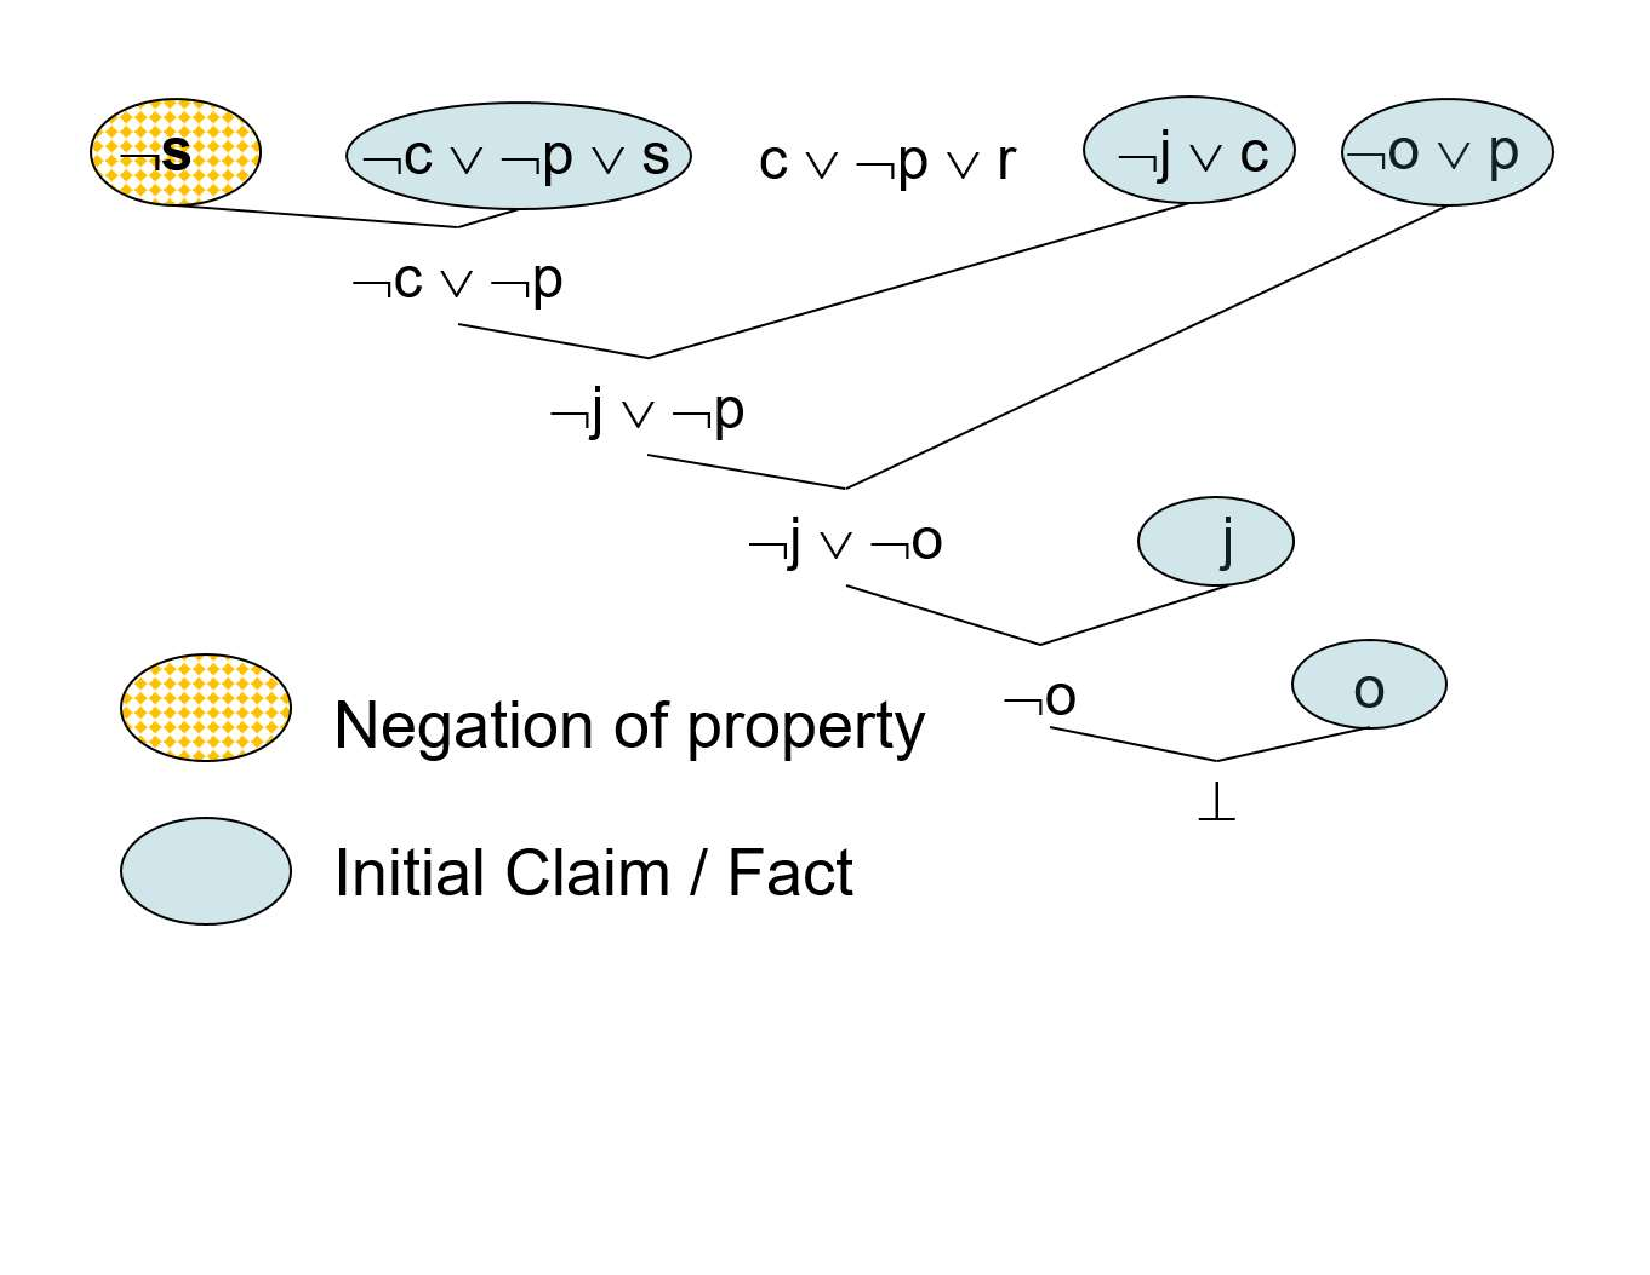
\includegraphics[width=\columnwidth]{images/proof.pdf}
%\caption{I will put a nicer picture}\label{fig:proof}
%\end{figure}
%
%To verify a requirement with respect to a model, SAT based model checkers like JKind, automatically constructs proofs of satisfaction. A proof can be visualized as a derivation tree where the leaves of the tree are axioms -- elements of the model such as components requirements, system assumptions -- and each interior node represents the application of an inference rule that leads to the claim, as shown in the Figure~\ref{fig:proof}. Our interest is to come up with an approach that will help extract the axioms that were necessary for the proof such that we can establish traceability to the requirements.
%
%While the proof generated by model checkers are typically invisible, SAT based model checkers allow users to query which axioms were used as part of the proof. We call the result to such a query, {\em inductive validity core} (IVC). The IVC helps explain how the solver reported the satisfaction of the requirement, that is comparable to the counterexample explains the negative result. In a recent work, we proposed a generic and efficient mechanism to extract the IVC from the proofs of requirements using inductive techniques. In general, the IVC extracted is not guaranteed to be contain only the necessary axioms, depending on how the model checker constructed the proof. Hence, in our approach after extracting the IVC we minimize it by recursively reducing them and checking if the remaining axioms are the necessary elements for the proof. Further, when induction is involved, many requirements are not themselves inductively provable and hence proof techniques introduce lemmas as part of the solving process in order to strengthen those requirements and make them inductive. The novelty of our approach is its efficient, accurate, and precise extraction of a minimum IVC in the presence of such auxiliary lemmas.
%
%In the next section we explain our approach to using the IVC to establish traceability between the requirements and actual parts of the model in a way that is useful to the user.



%
%
%
%
%Our aim is to establish requirements traceability by leveraging the capability of the sophisticated model based tools. \anitha{editing.....}
%
%
%However, with the increase in the size and complexity of the models, it is not easy to understand how and where the requirements are implemented in the models.
%
%
%Such as an association between the requirements and the model, in other words traceability, helps effectively perform :
%\begin{itemize}
%  \item \textbf{Impact analysis} - To determine which parts of the model implements the requirement, how a change in requirement affects the model and check if all requirements are implemented by its components.
%  \item \textbf{Dependency analysis} -  To identify which requirement had given rise to specific parts of the model, identify which requirement will be affected if the component is changed, assess the coverage of the requirements over the model, determine which parts of the components do not trace to any requirement.
%\end{itemize}
%
%
%
%Our interest is to be able to establish requirements traceability in the context of model based development (MBD), in which the systems are modeled using some form of mathematical notations. MBD is emerging as a widely accepted technique to developing systems, especially safety critical systems and has been very successful in identifying errors early in the development cycle and help improve the quality of the system.
%
%
%
%\textbf{Existing MBD traceability techniques.}Unfortunately, one of the major challenges in MDB is precisely that traceability. The main reason behind the difficulty is the inherent complexity of the models that makes the process of manually establishing trace links exhausting. However, there has been some research efforts to automatically establish the traceability between requirements and model elements. Some of them include :
%\begin{itemize}
%  \item Event-Based Traceability (EBT) (Cleland-Huang et al) is a method that automatically establishes trace links and maintains it, between requirements to models, using event-based mechanisms.
%  \item Egyed and Grunbacher enhance the basis from which they derive links by following the approach of dynamic program analysis: They record program execution traces (these are—as described earlier—dynamic program behavior logs) from the execution of test-cases. They combine the results with a set of requirements-to-code traceability links, which have to be established manually beforehand and infer traceability links between requirements.
%  \item Wenzel et al. describe a tool which is able to compare the version history of models, to derive traceability links, and consequently, to reconstruct the evolution steps of single model elements.
%  \item I have a survey paper, I will fill more relevant work here
%\end{itemize}
%
%\textbf{SA is good technique for traceability.}While the above techniques establish trace links, without a sematic rationale, Satisfaction Arguments offer a meaningful way to establish traceability between functional requirements and its realization. Unlike traditional traceability that just links two artifacts, satisfaction arguments are aimed to provide an explanation to why the traceability was established. It has been recognised that establishing traceability using satisfaction arguments has been very useful.\anitha{I want to make this a single sentence to lead to our work.}
%
%
%
%
%
%\textbf{In previous work we} demonstrated an approach to system construction in which compositional proofs are used to to establish satisfaction arguments. Given an architectural model of the system (decomposition of system into components) in which each component (including the system) is endowed with its own behavioral requirements and assumptions it makes about its environment, our approach compositionally verifies if system level requirements as a logical consequence of the component level requirements. To implement our approach, we used a tool called AGREE \cite{NFM2012:CoGaMiWhLaLu} -- a compositional reasoning framework based on assume-guarantee reasoning ~\cite{McMillan99:circ}, that provides an appropriate mechanism for formally capturing the model of the system and verify system requirements.


    \section{Complete Traceability}
\label{sec:discussion}

Through formal definitions in the previous section we highlight two critical facets -- the semantics and completeness -- in establishing traceability. In our experience, we found that just being able to trace a requirement to a target artifact that satisfies it, say a line of code, is not useful; a holistic view of how that line of code in conjunction with other related lines of code satisfy the requirement provides meaningful information to perform analysis such as assessing the impact of a change. By defining a trace from requirements to the set of target artifacts, we advocate that traceability be captured in a way that upholds its semantic rationale. Further, we also found that many analyses that are performed using sets of trace links without a clear picture whether the trace links are adequate for the purpose.\mike{Which analyses are we talking about here?  This seems like a bold, and unsupported claim.}  By considering $SOS$ trace links and complete traces for each requirement, we can assess analyses related to requirements satisfaction traceability on a proper semantic foundation.  In this section, we elaborate on how the semantic foundations in the previous section help us understand, assess, and use traceability precisely.

%that we explain in the previous section not only provides an in-depth understanding of how the system satisfies requirements but acts as a metric to assess the quality of traceability established for a system and enhances the precision of analysis using the traceability information.

\subsection{Categorizing the Set of Support}

Establishing $ASOS$ for a requirement, one gets a clear picture of the all possible ways that requirement is satisfied. This information helps categorize each target artifact into one of the following groups for that requirement.  The relationships are illustrated graphically in Figure~\ref{fig:maymust}, and explained formally below.
\begin{itemize}
  \item \textbf{MUST} elements - the target artifacts that are present in all the sets of support for a requirement (black triangles in Figure~\ref{fig:maymust}).
      %$$ MUST_x = \{\forall i (S_xi \in \Sigma_x) \mid \bigcap S_xi \}$$
      $$ MUST (r) = \bigcap \ ASOS(r) $$

  \item \textbf{MAY} elements - target artifacts that are used in some, but not all, sets of support (red dots in Figure~\ref{fig:maymust}).
      $$MAY(r) = (\bigcup ASOS (r)) \setminus MUST (r) $$

  \item \textbf{IRRELEVANT} elements - target artifacts that are not in any of the set of support (green stars in Figure~\ref{fig:maymust}). $$IRR(r) = I \setminus (\bigcup ASOS (r))$$
\end{itemize}

\begin{figure}[htb]
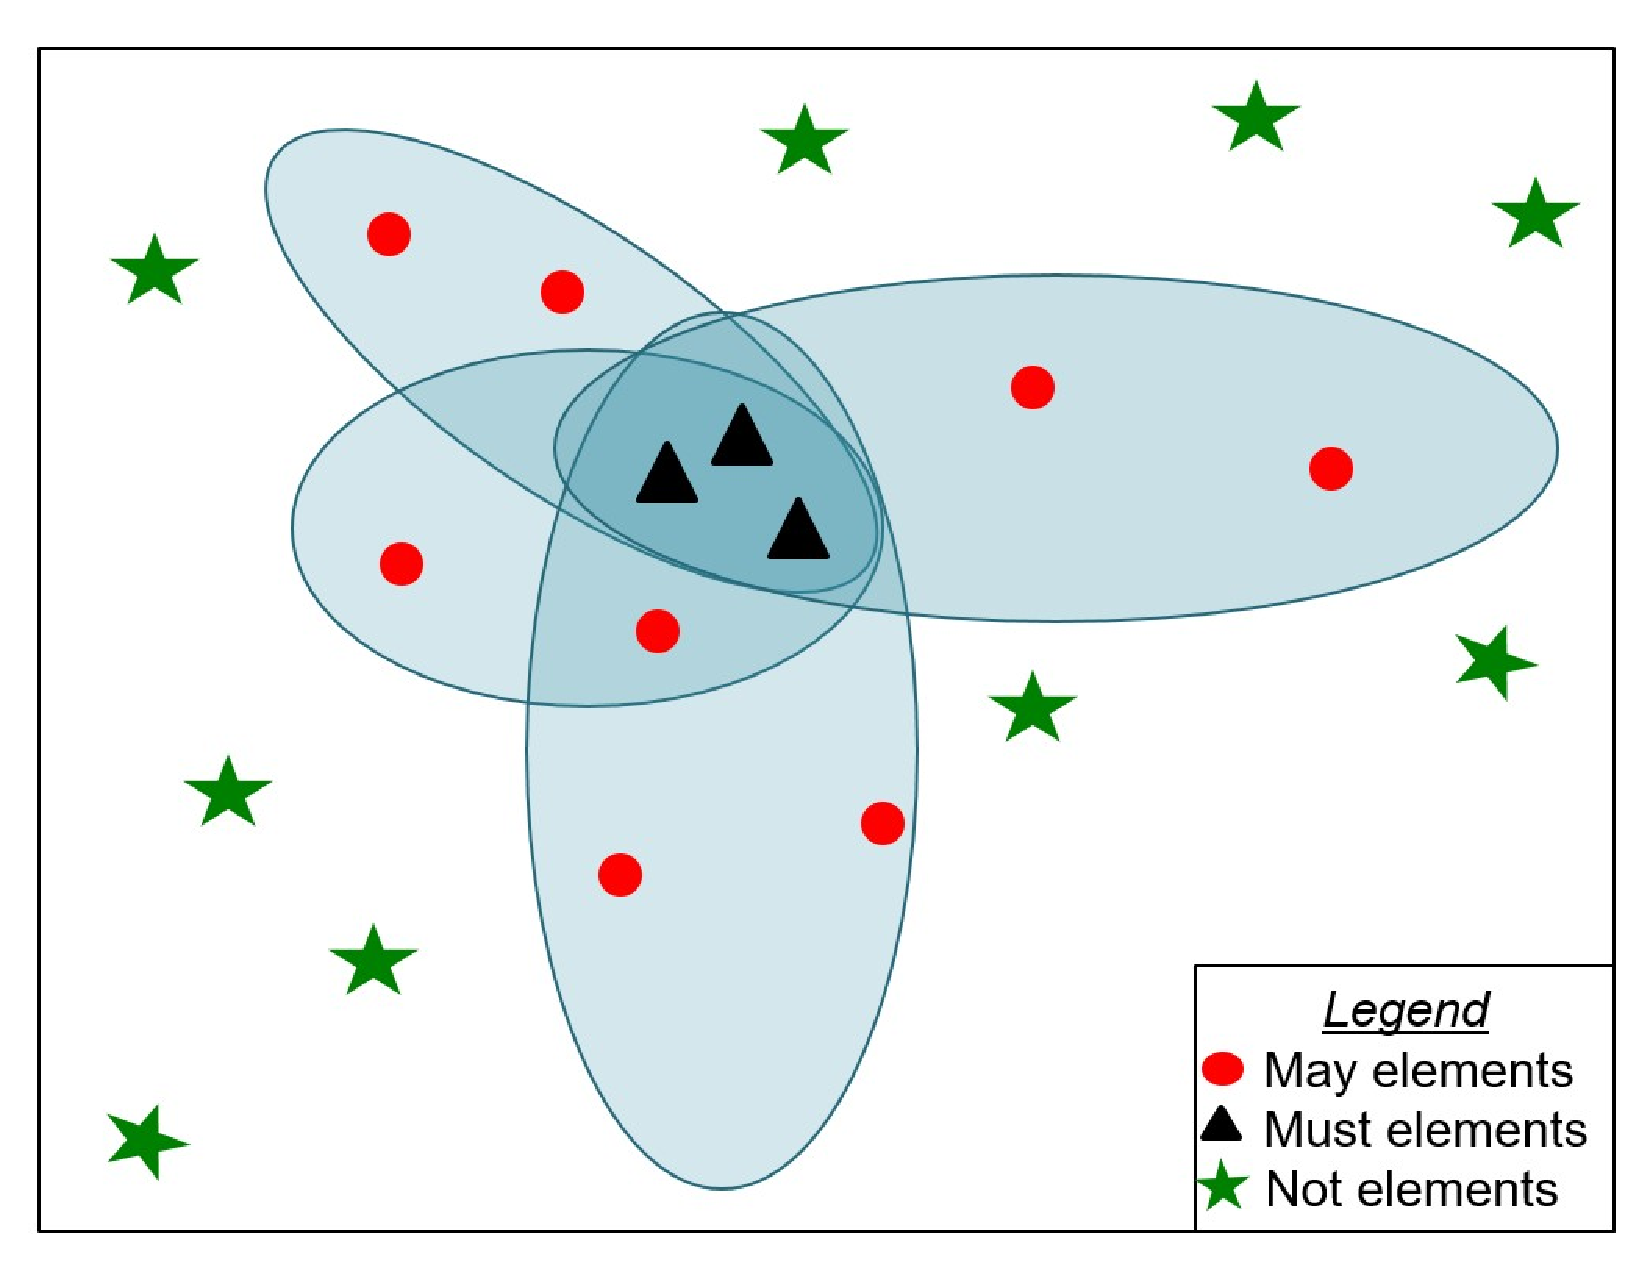
\includegraphics[width=\columnwidth]{images/may_must.pdf}
\caption{May - Must - Irrelevant Set of Support}\label{fig:maymust}
\end{figure}

This categorization helps identify the role and relevance of each target artifact in satisfying a requirement. The MUST elements are those target artifacts that are absolutely necessary for the requirement satisfaction. Hence, any change to these elements will most likely impact on each other. On the other hand, MAY elements indicate those target artifacts that satisfy the requirement in one of the possible ways.  Any change to just one of these elements will not affect the satisfaction of that requirement. The IRRELEVANT elements are never required to satisfy the requirement, so neither does a change in these artifacts affect the satisfaction of the requirement, nor does a change in the requirement necessitate a change in these elements (at least in terms of satisfaction).


\subsection{Using Traces for Precise Analysis}

The categorization of the set of support to be useful in several analyses:

\paragraph{Impact Analysis}: The $ASOS$ set improves understanding of how a change in the requirement change will affect the target artifacts and vice versa. This categorization precisely helps identify those parts of the system that definitely have to change when there is a change in requirement. MUST elements are those target artifacts that are highly likely to change with any change in the requirement, whereas not all MAY elements may need to be changed. On the other hand, if a MUST set is empty -- there are no common target artifacts between the sets of support -- it indicates that the requirement has been (intentionally or unintentionally) implemented in independent ways, such as fault tolerant systems. 



If we examine all the sets of support for all requirements and categorize them, then the elements in the MUST set describe target artifacts that are critical for all requirements~\mike{should we characterize this formally?}.  %This helps assess how a change in one element may affect other requirements.


If we examine changing a target artifact, if it appears in the MUST set for any requirement, then this requirement must be re-verified.  However, if it appears in the MAY set for the requirement, then we can instead remove any sets-of-support that contain the element; as long as there still exists at least one set of support for the requirement, no reverification is necessary.

%have to remove any SOS
%take each target artifact and trace to the requirements it satisfies, one can get clear idea about all the requirements it satisfies. If we decide to change a target artifact as long as it is not in any of the MUST sets for any requirement, it becomes evident that it will not affect the satisfaction of any requirement.

\paragraph{Verification and Validation}

Complete traceability can assist in tailoring verification and validation in systems. For instance, if several requirements have a certain target artifact in their MUST set, say an particular assumption, it reveals the importance of focusing V\&V attention on that artifact. Along the same lines, for a system with a complex architecture (components that each have functionality) such as  system of systems, this categorization helps identify components that is critical to satisfy most requirements. This helps plan verification strategies.

Further, the notion of complete traces helps to assess if requirements are satisfied by the system in an unintended manner. It is well known that issues such as vacuity~\cite{Kupferman03:Vacuity} can cause requirements to be satisfied in a trivial manner. Even for non-vacuous requirements, it can be the case that requirements can be satisfied using a much smaller portion of the system than intended because they are incorrectly specified.  By capturing all the set of support and categorizing them, it is possible to examine whether the MUST set corresponds to expectations on the system, or, if more rigor is required, to examine each set of support individually to see whether it matches expectations.
%one could evaluate if there are unintended target artifacts that might cause the requirements to be satisfied. %In one of our experiments using an infusion pump system software, while capturing the $RST_m$ for a requirement we discovered that there was a requirement whose set of support included a not the one that  to be trivially satisfied. When we

\paragraph{Completeness Checking}

By getting all the sets of support for all requirements of the system and categorizing them,  it gives a clear picture about the role of target artifacts in satisfying the requirement.  By reversing the direction of the complete requirement satisfaction trace, one can find if there are target artifacts that do not trace to any requirement.  This can be performed by examining the minimal set of target elements used by {\em any} SOS for {\em all} requirements.  If so,  it is a possible indication of ``gold plating" or missing requirements. In other words, it helps assess if there requirements of the system are completely specified with respect to describing all the behaviors of the system. Being able to assess the coverage of requirements over the model is crucial in the safety critical system domain.

\paragraph{Comparing Traceability Approaches}
%\anitha{I am not happy with this now.... But I do want to say something along these lines... }
%\mike{I agree, but I have not made any changes to the section.}
There is substantial interest within the Requirements Engineering research community (and our immediate research group) towards automating the construction and maintenance of traceability links.  To that end, there are repositories such as \mike{Name of Jane's repository HERE + citation} containing many example systems, each with a reasonably complete set of requirements and target artifacts and with trace links constructed by groups of experts.  It is then possible to benchmark automated and semi-automated traceability approaches against vetted sets of trace links.

We are, in general, very supportive of this approach: benchmarking against a reasonable set of candidate models has been very important in several areas of computer science research, including CPU, GPU, and compiler performance~\mike{citations here}, performance of SAT/SMT solvers and model checkers~\mike{cite SATcomp and SMTcomp}, and many other areas.  However, it can also be misleading if the benchmark problems are not carefully selected or if results are incorrectly computed, as described in, e.g., several articles critical of benchmarking for CPU/GPU performance~\mike{citations here}.

For traceability research, the usual standard measures for examining the performance of different approaches is in terms of {\em precision} and {\em recall} against the ``gold standard'' set of traceability links that exist in repositories.  Our concern is that, for requirements satisfaction traceability, there are often many such sets of valid links, as we have explored in this paper, so these metrics may be misleading.  One can envision situations in which the gold standard pursues one set of support and the automated approach pursues another, leading to low precision and recall scores.  A close examination of traceability links and categorizations such as the ones we have explored may be useful to provide more accurate measurements of the quality of automated approaches.  If requirements have more than one SOS, the gold standard should probably contain each of these arguments.  In addition, the ability to characterize trace links as $MAY$ or $MUST$ may be a fruitful direction of future research for automated approaches to constructing trace links.


%To the best of our knowledge, the existing benchmarks and ways to establish benchmarks to assess the effectiveness of traceability techniques or evaluate the trace links is not guaranteed to be flawless. The correctness and thoroughness of the benchmarks are in someway assumed and not rigorously assessed. A number of research work compute the precision and recall of their traceability approaches by using such benchmarks. We believe that to evaluate the completeness and precision of those benchmarks we need to first rigorously characterize it. The requirements satisfaction trace defined in the previous section helps us move forward in that direction. Since the trace is based on establishing a satisfaction argument it is straightforward to verify/validate the precision of each trace (which is 100$\%$). The complete requirements satisfaction trace, as the name suggests, is defined to capture traces to all sets of support. While this may sound theoretical, once established it will be the perfect benchmark to compare results to.

\mike{Stopped here.  Not sure we want the discussion below at all.}
Contrary to the general notion that it is impossible or extraordinarily difficult to identify all trace link in practice~\cite{stravsunskas2002traceability}, some of the initial results from our recent efforts~\cite{IVCTechReport} indicate that such complete requirements satisfaction trace can be established, in fact automatically in the realm of formal methods and model based developments. In the next section, we breifely describe our prior work and our plans to extend it to establish complete traceability. While the details the approach and initial results are not in scope of this paper, an interested reader is directed to~\cite{IVCTechReport}.



%
%
%
%\newcommand{\bfalg}{IVC\_BF}
%\newcommand{\ucalg}{IVC\_UC}
%\newcommand{\ucbfalg}{IVC\_UCBF}
%
%The approach from the previous section establishes trace links between properties at different levels of the system architecture based on inductive validity cores derived from inductive proofs.  For functional requirements, this approach automates the traceability information necessary to establish {\em satisfaction arguments} in the style of \mike{Ref to Will it Work HERE}.  In so doing, it allows a substantial change in how traceability is performed, and to some extent, what traceability {\em means}.  As we explained in the motivating example, there is often more than one way that the requirements could be satisfied by the model, that is, there is more than one set of support for the requirement.  This requires an examination of how we perceive traceability in terms of which model elements (equivalently: subcomponent properties) are {\em always required} by any proof, which elements are {\em sometimes required}, and which elements are never required, which we call {\em must} and {\em may} trace links.  It also brings up fruitful discussions on how architectures are constructed and the nature of the links between requirements and architecture.
%
%\subsection{Overhead of Computing IVCs and Minimality of Generated IVCss}
%In our accompanying technical report~\cite{}, we present two algorithms that are used to compute IVCs and an experiment to examine the quality of the approach.  Our primary concerns are the {\em efficiency} and {\em
%minimality} of the approach.  Efficiency is computed in terms of wall-clock time: how much overhead does the IVC algorithm introduce?  Minimality is determined by the size of the IVC: cores with a smaller number of
%variables are preferred to cores with a larger number of variables.  Both of the proposed algorithms are {\em sound}, in the sense that from the IVC, it is always possible to reconstruct the proof, so they do not miss trace links.
%
%In~\cite{}, we present two algorithms that pose different tradeoffs between these goals.  The first algorithm, called \ucalg, uses UNSAT cores to determine an IVC and runs very efficiently (on average, for the 477 models in the experiment, about 15\% overhead over performing the proof when using the z3~\cite{} solver), but is not guaranteed to yield a minimal IVC; on average, it yields a core that is 21\% larger than minimal.  The second algorithm, called \ucbfalg, adds a ``brute force'' postprocessing stage that guarantees that the generated core is minimal, but adds, on average, a greater than 30-times slowdown to the proof.
%
%\subsection{On-Demand Traceability}
%
%Because the efficient algorithm (\ucalg) adds very little overhead to the model-checking process, which is itself quite efficient, we can think of it as providing ``on-demand'' traceability.  In most traceability approaches, maintenance of trace links is a very significant concern and one of the reasons that finding and fixing errors is so expensive in critical systems.  However, with our approach, it is straightforward to provide users with accurate trace information consistent with the model immediately after changes are made.  This allows traceability to easily be used as an {\em exploratory} analysis early during requirements gathering and architectural prototyping.  We have used it in this way in the DARPA SOSITE project, where we used traceability information to check whether we were writing appropriate requirements and to check ``semantic vacuity'', as will be described in a following section.
%
%In hand-generated trace links for satisfaction, there is a potential for both missing required traceability links and addition unnecessary traceability links.  In our approach, there is an interesting tradeoff in terms of usability of trace links: is it more important that they are inexpensive to generate or that they are minimal?  In our approach, for functional requirements, if we overapproximate the set of required model elements, does this still provide value?  Our claim of (on average) 21\% larger sets of support is perhaps misleading: for the GPCA models, which contain hundreds of possible subcomponent requirements that contribute to a proof, the \ucalg\ set of support is either the same as the \ucbfalg, or it has between 1 and 5 extra elements (e.g., 10 elements vs. 8 elements).  For users seeking to understand the relationships between system and subcomponent requirements, it seems that the faster algorithm may yield reasonable results.  On the other hand, if we want to use the tool for some kind of certification-related activity, it is likely worth the extra cost to get more exact results.
%
%\mike{more here???}

%\subsection{Categorizing Trace Links}
%We often describe ``the'' traceability matrix for a system, tracing requirements to lower-level requirements, design artifacts, or implementations.  However, at least for functional requirements, it is more correct to speak of ``a'' traceability matrix, because there are multiple minimal sets of model elements that lead to a proof.
%
%
%For instance, in safety critical system domain for fault tolerance one could intentionally add multiple ways to satisfy a requirement, or one could unintentionally add model functionality that leads to multiple ways of satisfying a requirement. By iteratively using our approach to query the solver for different sets of support until it does not find any, we can obtain all the sets of support for a requirement. Getting all the sets of support is nothing but establishing complete traceability between the requirements and all the parts of the model that contribute to satisfying it.
%
%%\subsection{Categorizing Support Elements}
%
%Establishing complete traceability paves way to indepth understanding of the model. Given all sets of support for a requirement, one could categorize them into the following, as illustrated in Figure~\ref{fig:maymust}:
%\begin{itemize}
%  \item MUST elements - support elements that are present in all the sets of support
%  \item MAY elements -  elements in set of support, but not common to all the sets of support
%  \item IRRELEVANT elements -  support elements of the model that are not in any of the set of support
%\end{itemize}
%
%\begin{figure}[htb]
%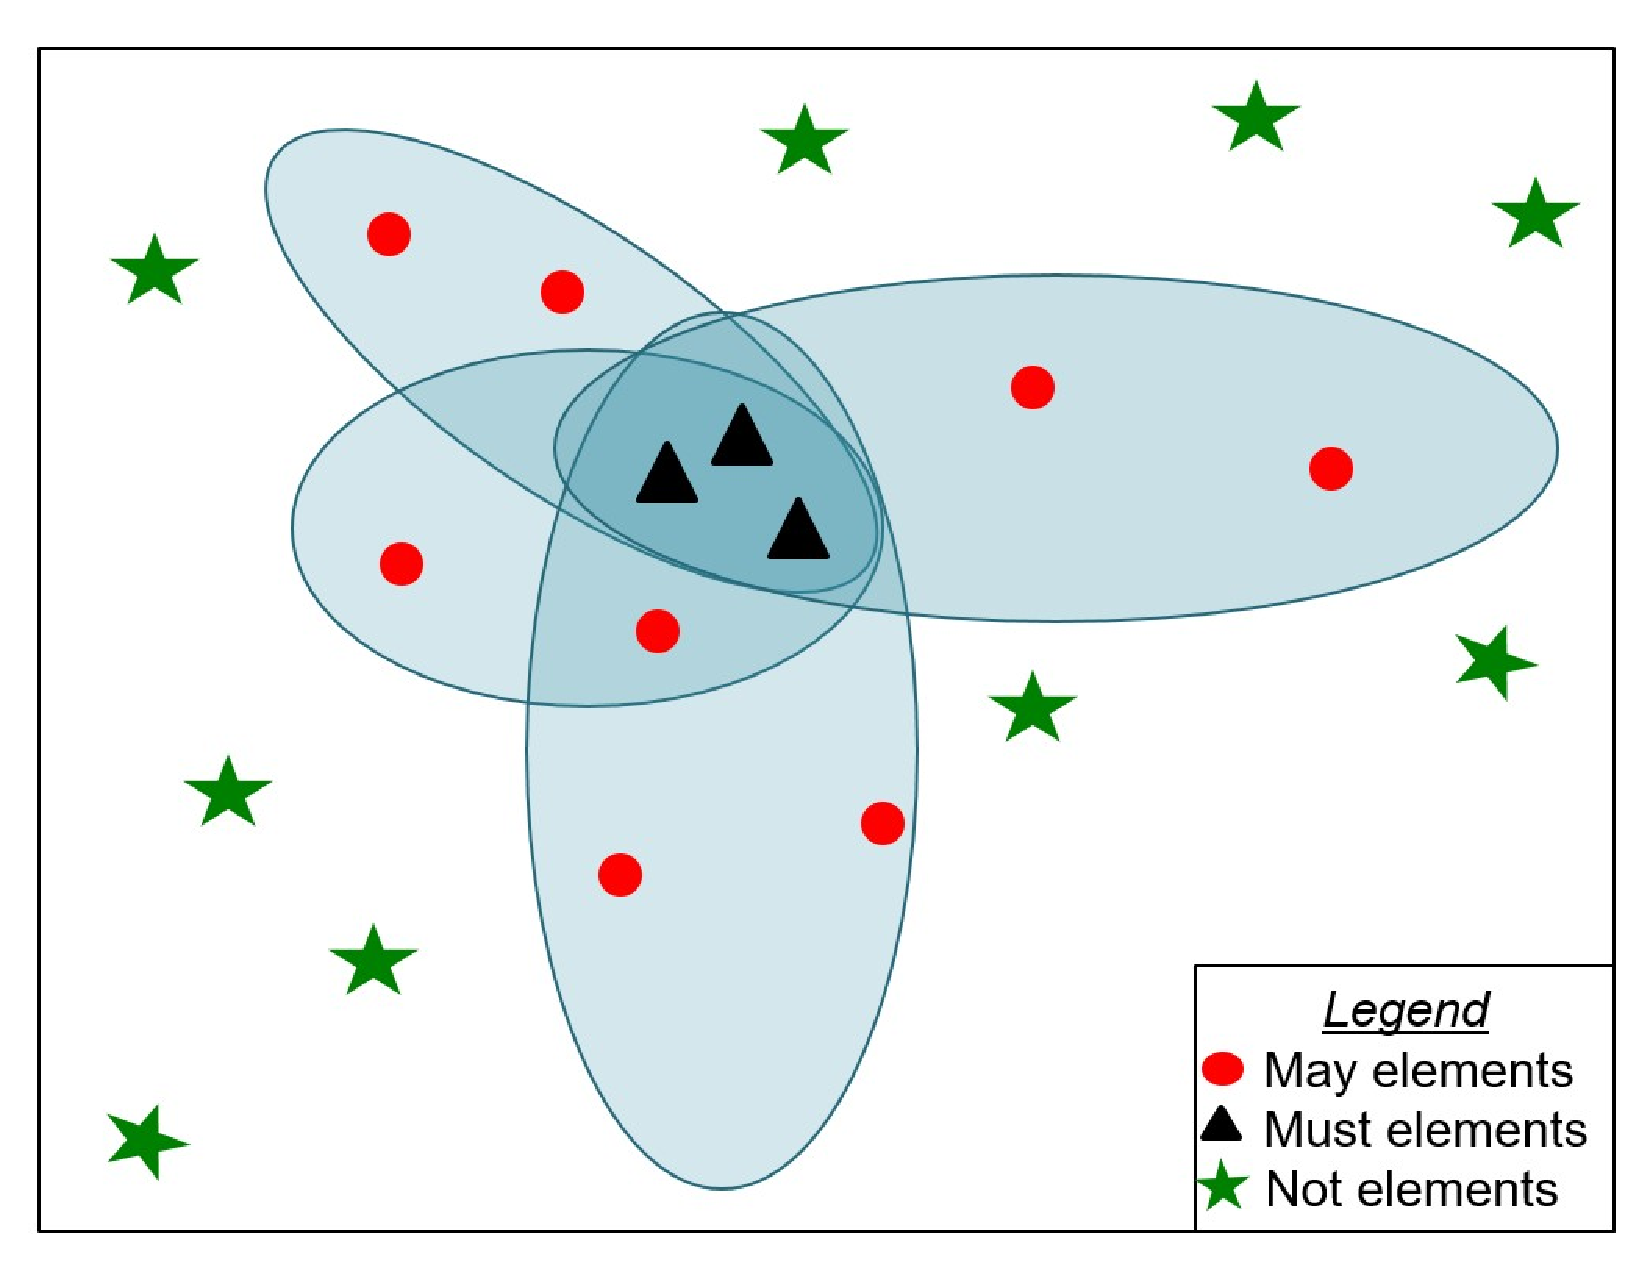
\includegraphics[width=\columnwidth]{images/may_must.pdf}
%\caption{May - Must - Irrelevant Set of Support}\label{fig:maymust}
%\end{figure}
%
%The MUST elements indicate that those parts of the model are absolutely necessary for the requirement to be satisfied. Hence, any change to either requirements or one of these elements will have an impact on the other. On the other hand, MAY elements indicate the parts of the model that satisfy the requirement in one of the possible ways. Any change to just one of these elements will not affect the satisfaction of the requirements. The NOT elements are in no way related to satisfying the requirements. When performing impact analysis of a change in requirements or dependency analysis to assess the effect of changing the model, this traceability provides a complete picture of all the dependencies.
%
%
%



%
%
%\subsection{Traceability Coverage}
%
%While establishing complete traceability is useful, to the best of our knowledge, how elaborately should traceability be captured is not well discussed in the literature. The question is "Should traceability be quantified?" The usual trace relationships between the system (or its model) and the requirements is "satisfies" or "implements" etc. We recommend that the relationship explicitly state whether traceability captures "one way to satisfy/implement" or "all the ways to satisfy/implement" the requirements. Making it explicit helps precisely realize the benefits of traceability.
%
%\anitha{in progress.}....


    \section{Discussion}

While the notion of correctness and completeness in requirements traceability is not a new topic of discussion, our argument is that it is not been rigorously defined and assessed. The intent of this RE@Next! paper is to clarify the foundations of tracing requirements to its realization - in particular the requirements satisfaction traceability -- and explaining its the benefits and ramifications.

While there are enormous amount work in the area of requirements traceability, there are no, to the best of our knowledge, rigours yardsticks or metrics to quantitatively and qualitatively access the trace links. This raises a qualm about the way traceability is assessed. Hence, we believe that there is a strong need to identify metrics, define approaches and develop tools that will rigorously assess trace links.

In this paper we define a strong theoretical framework to understand and assess requirements satisfaction traceability, that we believe is an initial attempt towards addressing the above need. By defining a requirements satisfaction trace from a requirement to a set of support, rather than a target artifact, we intertwine the rationale to verify/validate its correctness automatically. Such traces are self-sufficient to be verified for correctness, without the need for another source of truth or spending enormous amount of time to validate them. By examining these traces one could verify and validate if the system indeed satisfies the requirements in s intended ways. Further, this helps redefine the notion of completeness in traceability from capturing trace links to all requirements to capturing *all* trace links to all requirements. It is worth reiterating that our goal is not yet another formalization of traceability but to provide the foundation for any future research on satisfaction trace link generation and assessment.

Contrary to the general notion that it is impossible or extraordinarily difficult to identify all trace link in practice~\cite{stravsunskas2002traceability}, some of the initial results from our recent efforts~\cite{2016arXiv160304276G} indicate that such complete requirements satisfaction trace can be established, in fact automatically in the realm of formal methods and model based developments. 



While the details the approach and initial results are not in scope of this paper, an interested reader is directed to~\cite{2016arXiv160304276G}.


%    \section{Background}
\label{sec:background}

%\newcommand{\bool}{\mathit{bool}}
\newcommand{\reach}{\mathit{R}}
\newcommand{\ite}[3]{\mathit{if}\ {#1}\ \mathit{then}\ {#2}\ \mathit{else}\ {#3}}

In order to discuss traceability with respect to satisfaction arguments, we introduce a simple formal model to describe it precisely.  In this model, a safety property $P$ represents a system requirement, and a transition system $(I, T)$, described below, represents an implementation.  Transition systems are abstract representations that can be used to describe any kind of implementation.\mike{note: we could also generalize $P$ from a safety property to any kind of property by parameterizing the notion of ``satisfaction'' $\vdash$}


\subsection{Transition Systems and Inductive Validity Cores\footnote{This Section is Extracted  from~\cite{IVCTechReport} } }

Given a state space $S$, a transition system $(I,T)$ consists of an
initial state predicate $I : S \to \bool$ and a transition step
predicate $T : S \times S \to \bool$. We define the notion of
reachability for $(I, T)$ as the smallest predicate $\reach : S \to
\bool$ which satisfies the following formulas:
\begin{gather*}
  \forall s.~ I(s) \Rightarrow \reach(s) \\
  \forall s, s'.~ \reach(s) \land T(s, s') \Rightarrow \reach(s')
\end{gather*}
A safety property $P : S \to \bool$ is a state predicate. A safety
property $P$ holds on a transition system $(I, T)$ if it holds on all
reachable states, i.e., $\forall s.~ \reach(s) \Rightarrow P(s)$,
written as $\reach \Rightarrow P$ for short. When this is the case, we
write $(I, T)\vdash P$.

We next define {\em validity cores}, which describe minimal portions of the transition relation $T$ necessary to construct a proof\footnote{In~\cite{IVCTechReport}, these are called inductive validity cores, because of the mechanism of proof used by the model checker for transition relations}.  Without loss of generality, we assume the
transition relation of the system has the structure of a top-level
conjunction. Given $T(s, s') = T_1(s, s')
\land \cdots \land T_n(s, s')$ we will write $T = T_1 \land \cdots
\land T_n$ for short. By further abuse of notation we will identify
$T$ with the set of its top-level conjuncts. %Thus we will write $x \in
%T$ to mean that $x$ is a top-level conjunct of $T$. 
Thus, we will write $S
\subseteq T$ to mean that all top-level conjuncts of $S$ are top-level
conjuncts of $T$. %We will write $T \setminus \{x\}$ to mean that $T$
%with the top-level conjunct $x$ removed. We will use the same notation
%when working with sets of invariants.

\begin{definition}{\emph{Validity Core:}}
  \label{def:ivc}
  Let $(I, T)$ be a transition system and let $P$ be a
  safety property with $(I, T)\vdash P$. We say $S \subseteq
  T$ is a {\em validity core} for $(I, T)\vdash P$ iff $(I,
  S) \vdash P$. When $I$, $T$, and $P$ can be inferred from
  context we will simply say $S$ is a validity core.
\end{definition}

\begin{definition}{\emph{Minimal Validity Core:}}
  \label{def:minimal-ivc}
  A validity core $S$ for $(I, T)\vdash P$ is minimal iff
  there does not exist $M \subset S$ such that $M$ is a validity core
  for $(I, T)\vdash P$.
\end{definition}

Note that minimal validity cores are not necessarily unique; there are often different ways that one can construct a proof using different parts of the transition system.  This insight guides the remainder of the paper~\mike{continue here...}

%While precise and complete traceability is beneficial but has been considered impossible to establish in practice~\cite{stravsunskas2002traceability}, our hypothesis is that, in the realm of model based development (MBD), it can be achieved in an automated and efficient manner. We base our hypothesis on the fact that in MBD, the artifacts - both models and requirements - are captured using some form of formal notation and sophisticated tools automatically verify if the requirements are satisfied in the models. We believe that the mathematics underlying the verification tools can be leveraged to establish traceability. In this section, we briefly explain some of our prior work that lead us to pursue our hypothesis.
%
%
%\subsection{System Modeling and Verification}
%
%Previously~\cite{hilt2013}, we demonstrated a model based approach to system construction in which compositional proofs are used to to establish satisfaction arguments. To cope with complexity of modeling and scalability of verification of large systems, we proposed an approach in which systems can be decomposed into subsystems, modeled individually and verified compositionally. The decomposition of system into subsystems induces the need to decompose the requirements of the system `flowed down'' to each subsystem that is then modeled and verified.
%
%Given an architectural model of the system (decomposition of system into components) in which each component (including the system) is endowed with its own set of requirements, we used a tool suite called AGREE~\cite{NFM2012:CoGaMiWhLaLu} -- a reasoning framework based on assume-guarantee reasoning~\cite{McMillan99:circ} -- to compositionally verify whether system level requirements are established as a logical consequence of the component level requirements and the system level assumptions. Using AGREE we were able to verify large and complex systems efficiently. AGREE partitions the task of verification along the architectural lines of the system. Stating from the leaf level, it systematically verifies if the parent level requirements hold as a logical consequence of its immediately child component requirements in the given architecture.
%
%To verify the requirements, AGREE uses a model checker called JKind~\cite{JKIND link}. JKind is an infinite-state model checker that is intended to verify functional requirements, in particular safety requirements. In the back-end, JKind uses an SMT solver such as Z3~\cite{DeMoura08:z3}, Yices~\cite{Dutertre06:yices}, MathSAT~\cite{Cimatti2013:MathSAT}, or SMTInterpol~\cite{Christ2012:SMTInterpol}.
%
%The underlying SMT solver automatically constructs proofs to establish satisfaction of requirements in the model. A proof can be visualized as a derivation tree where the leaves of the tree are axioms -- elements of the model such as components requirements, interface connections, system assumptions -- and each interior node represents the application of an inference rule that leads to proving the system requirement. If the solver encounters a violation of a requirement while constructing the proof, it reports it along with a counterexample - a concrete path of execution that explains the violation. On the other hand, when the proof is successfully constructed, the tool reports that the requirement is satisfied.
%
%
%\subsection{Inductive Invalidity Cores}
%
%While the above approach is very useful in proving system level requirements, in the event
%that requirement is proved, it is not always clear what level of assurance should be invested in the
%result.  Given that these kinds of analyses are typically performed for safety critical system, this
%can lead to overconfidence in the behavior of the fielded system. It is well known that issues such as
%vacuity~\cite{Kupferman03:Vacuity} can cause verification to succeed despite errors in a requirements
%or in the model. Even for non-vacuous requirements, it is possible to over-constrain the {\em
%environment} of the model such that the implementation will not work in the actual operating
%environment. Hence, to gain confidence over the verification we pursed an approach that would provide
%us with an evidence of the successful verification. An evidence in this context is nothing but an
%explanation about which parts of the model (the component requirements and system assumptions) the
%model checker used to prove the system level requirement.
%
%Since the solvers typically abstract away the proof it creates, we developed a novel technique to query the solver to excavate the axioms that were used as part of the proof. We call the result to such a query as the {\em inductive validity core} (IVC). The IVC helps explain how the solver reported the satisfaction of the requirement, that is comparable to the counterexample explains the negative result.
%
%Extracting the IVC was a significant step towards testing our hypothesis, but it was not sufficient, since the IVCs were not in a easily understandable format. In the process of verifying the requirements AGREE, JKind and the underlying solvers transform the original model into a number of intermediate models that no longer resemble the original model. The IVCs were parts of the transformed model that was not directly correlatable to the original model. Hence, to be understandable, the IVCs had to be linked back to parts of the original model. This was critical for establishing traceability that is meaningful. In the following section, we explain our approach to rigorously link the IVC to actual parts of the model to establish traceability between the requirements and the model.
%
%







%
%
%\subsection{System Modeling and AADL}
%
%Previously~\cite{hilt2013}, we demonstrated a model based approach to system construction in which compositional proofs are used to to establish satisfaction arguments. To cope with complexity of modeling and scalability of verification of large systems, we proposed an approach in which systems can be decomposed into subsystems, modeled individually and verified compositionally. The decomposition of system into subsystems induces the need to decompose the requirements of the system `flowed down'' to each subsystem that is then modeled and verified.
%
%To capture the decomposition of systems or architecture of interest and the requirements allocated to components, we use architectural models. The architectural models include components and component interfaces, interconnections between components, and requirements on the components.  Thus, the architectural models describe the interactions between components and their arrangement in the system.  By annotating them with requirements for component behavior, these models become a means to support iteration between requirements allocation and architectural design.  We use the Architecture Analysis and Description Language (AADL) to describe architectural models.  AADL includes constructs that describe both software and hardware components, as well as mapping software components to physical resources and the devices with which they communicate. Furthermore, it contains an extension mechanism (called an {\em annex}) that can be used to extend the language to support additional features, such as requirements modeling.
%
%\subsection{System Verification and AGREE/JKind}
%
%Given an architectural model of the system (decomposition of system into components) in which each component (including the system) is endowed with its own set of requirements, we used a tool suite called AGREE~\cite{NFM2012:CoGaMiWhLaLu} -- a reasoning framework based on assume-guarantee reasoning~\cite{McMillan99:circ} -- to compositionally verify whether system level requirements are established as a logical consequence of the component level requirements and the system level assumptions. Using AGREE we were able to verify large and complex systems efficiently. AGREE partitions the task of verification along the architectural lines of the system. Stating from the leaf level, it systematically verifies if the parent level requirements hold as a logical consequence of its immediately child component requirements in the given architecture.
%
%To verify the requirements, AGREE uses a model checker called JKind~\cite{JKIND link}. JKind is an infinite-state model checker that is intended to verify functional requirements, in particular safety requirements. JKind proves safety properties using multiple cooperative engines in parallel including $k$-induction~\cite{SheeranSS00}, property directed reachability~\cite{Een2011:PDR}, and template-based lemma generation~\cite{Kahsai2011}. JKind accepts Lustre programs written over the theory of linear integer and real arithmetic. In the back-end, JKind uses an SMT solver such as Z3~\cite{DeMoura08:z3}, Yices~\cite{Dutertre06:yices}, MathSAT~\cite{Cimatti2013:MathSAT}, or
%SMTInterpol~\cite{Christ2012:SMTInterpol}.
%
%The underlying SMT solver automatically tries to constructs proofs to establish satisfaction of requirements in the model. A proof can be visualized as a derivation tree where the leaves of the tree are axioms -- elements of the model such as components requirements, interface connections, system assumptions -- and each interior node represents the application of an inference rule that leads to proving the system requirement. If the solver encounters a violation of a requirement while constructing the proof, it reports it along with a counterexample - a concrete path of execution that explains the violation. On the other hand, when the proof is successfully constructed, the tool reports that the requirement is satisfied. %This approach was able to scalably verify large and complex systems.
%
%%\\begin{figure}[htb]
%%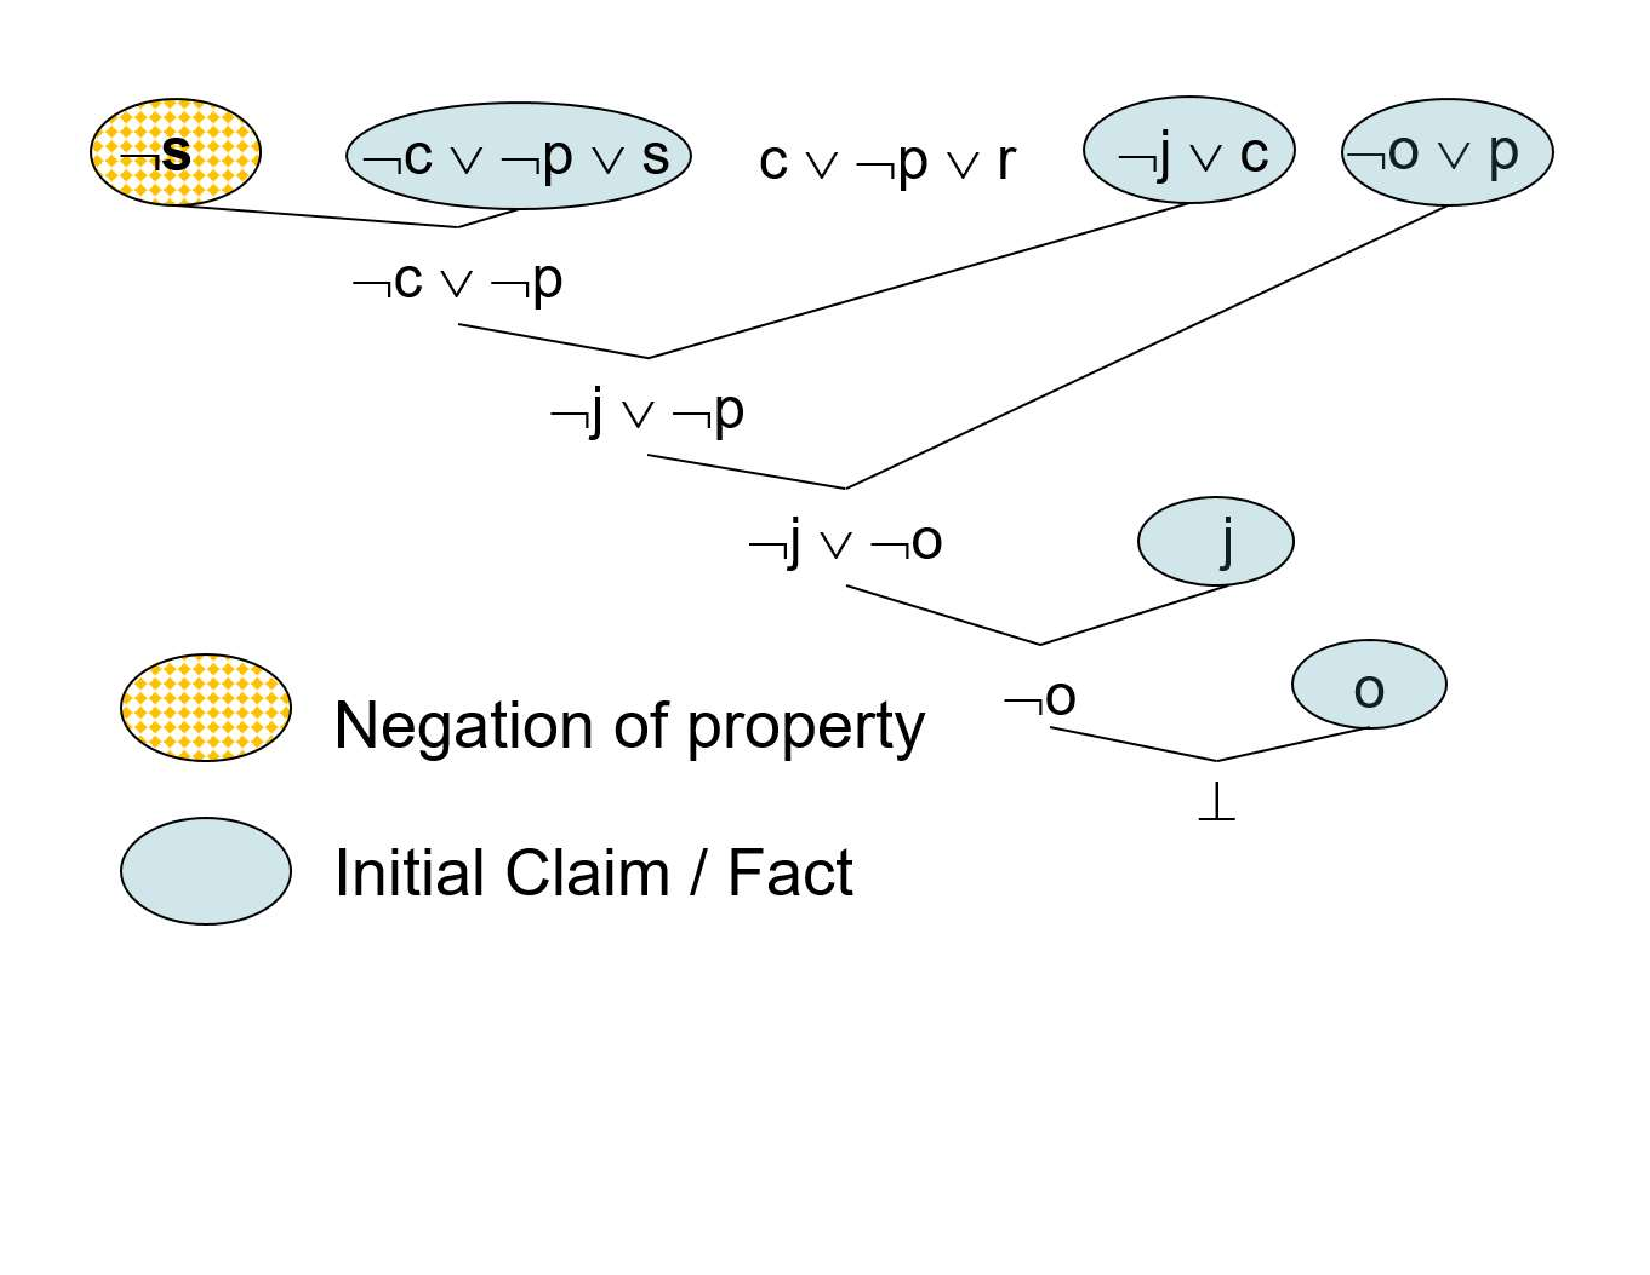
\includegraphics[width=\columnwidth]{images/proof.pdf}
%%\mike{This is not accurate w.r.t. JKind actually does for IVCs}
%%\caption{An accurate picture would be somewhat difficult.}\label{fig:proof}
%%\end{figure}
%
%\subsection{Inductive Invalidity Cores}
%
%While the above approach is very useful in proving system level requirements, in the event
%that requirement is proved, it is not always clear what level of assurance should be invested in the
%result.  Given that these kinds of analyses are typically performed for safety critical system, this
%can lead to overconfidence in the behavior of the fielded system. It is well known that issues such as
%vacuity~\cite{Kupferman03:Vacuity} can cause verification to succeed despite errors in a requirements
%or in the model. Even for non-vacuous requirements, it is possible to over-constrain the {\em
%environment} of the model such that the implementation will not work in the actual operating
%environment. Hence, to gain confidence over the verification we pursed an approach that would provide
%us with an evidence of the successful verification. An evidence in this context is nothing but an
%explanation about which parts of the model (the component requirements and system assumptions) the
%model checker used to prove the system level requirement.
%
%Since the solvers typically abstract away the proof it creates, we developed a novel technique to query the solver to excavate the axioms that were used as part of the proof. We call the result to such a query as the {\em inductive validity core} (IVC). The IVC helps explain how the solver reported the satisfaction of the requirement, that is comparable to the counterexample explains the negative result. In general, the IVC extracted is not guaranteed to be contain only the necessary axioms, depending on how the model checker constructed the proof. Hence, in our approach after
%extracting the IVC we minimize it by recursively reducing them and checking if the remaining axioms are
%the necessary elements for the proof. Further, when induction is involved, many requirements are not
%themselves inductively provable and hence proof techniques introduce lemmas as part of the solving
%process in order to strengthen those requirements and make them inductive. The novelty of our approach
%is its efficient, accurate, and precise extraction of a minimum IVC in the presence of such auxiliary
%lemmas.
%
%Extracting the IVC was a significant step towards testing our hypothesis, but it was not sufficient, since the IVCs were not in a easily understandable format. In the process of verifying the requirements AGREE, JKind and the underlying solvers transform the original model into a number of intermediate models that no longer resemble the original model. The IVCs were parts of the transformed model that was not directly correlatable to the original model. Hence, to be understandable, the IVCs had to be linked back to parts of the original model. This was critical for establishing traceability that is meaningful. In the following section, we explain our approach to rigorously link the IVC to actual parts of the model to establish traceability between the requirements and the model.

%    \section{Related Work}

The intent of this section is to explain related work for traceability model based developments.

    \section{Conclusion}




%\section{Related Work}
%
%Establishing traceability, especially in MDB is not a new topic, but has
%
%One of the major challenges in MDB is precisely establishing traceability between the system requirements and the parts of the model that implements it. The main reason behind the difficulty is the inherent complexity of the models that makes the process of manually establishing trace links exhausting. However, there has been some research efforts to automatically establish the traceability between requirements and model elements. Some of them include :
%\begin{itemize}
%  \item Event-Based Traceability (EBT) (Cleland-Huang et al) is a method that automatically establishes trace links and maintains it, between requirements to models, using event-based mechanisms.
%  \item Egyed and Grunbacher enhance the basis from which they derive links by following the approach of dynamic program analysis: They record program execution traces (these are—as described earlier—dynamic program behavior logs) from the execution of test-cases. They combine the results with a set of requirements-to-code traceability links, which have to be established manually beforehand and infer traceability links between requirements.
%  \item Wenzel et al. describe a tool which is able to compare the version history of models, to derive traceability links, and consequently, to reconstruct the evolution steps of single model elements.
%  \item alloy work here or at the end?
%\end{itemize}
%\anitha{I have a survey paper, I will fill in relevant work here}
%
%While the above techniques establish trace links, without a rationale for why and how they were established they are often inadequate to perform useful analysis in practice~\cite{Trace links explained: An automated approach for generating rationales}. In that context, \textbf{\emph{Satisfaction Arguments}} offer a meaningful way to establish traceability between functional requirements and its realization. Originally proposed by Zave and Jackson, satisfaction argument is an approach to demonstrate how the behaviours of the system along with the assumptions made about its environment satisfy the functional requirements. These arguments have been enormously useful in establishing traceability between the requirements and parts of the system that implements them. Unlike traditional traceability that just links two artifacts, satisfaction argument is aimed to provide an explanation to why the traceability was established.


%    \input{hrrmodel}
%    \input{caseexample}

%
\begin{enumerate}

  \item Requirements traceability is the association that is established between the requirements and other development artifacts in the system such as design, code, test cases etc.

  \item Such traceability information has a number of uses. Impact analysis, Dependency analysis and satisfaction argument etc. Give example for each.

  \item Our focus in this paper is discussing requirements traceability in the context of MBD

  \item MDB is taking off in the safety critical system domain, in which models of the system are developed using tools such as Simulink, Stateflow etc. This has been a very successful development technique since it helps identify errors early in the development cycle.

  \item However, with increase in complexity of the developed models it is not easily discernible to identify how and where the requirements are in the models. In fact, to cope with complexity, it has been a common practices to decompose the task of modeling the entire sysstem into smaller and manageable parts, that are individually developed and verified and then they are composed using some technique to ensure if they are satisfied. How and where the requirements are implemented in the models is not easy to see.

  \item In this context, We believe that traceability in MBD between requirements and models is highly beneficial for various purposes...

  \item Our hypothesis is that by leveraging the capability of the tools that verify requirements, we can establish trace links between the requirements and the model. In this paper, we elaborate on our first successful attempt in validating our hypothesis.

  \item In previous work, using compositional verification techniques we verified if the system level requirements of system that is decomposed into components, is satisfied by its component level requirements given the system level assumptions. We used a compositional reasoning tool, \textbf{AGREE}.

  \item The tool produces a proof of correctness for the system level requirements, whose claims are nothing but the component level requirements and system level assumptions. By extracting the claims, we get what we call "set of support", the necessary elements for the proof. This set of support is nothing but those component requirements and assumptions that contributed to satisfying the requirement. The

  \item While one set of support is one way the model satisfies the requirement. it is interesting to know if there are more than one set of support. To our surprise Yes. Then, if we get all possible trace links, then what we get is a complete traceability between models and requirements.

  %\item the intent of this paper is not explain the implementation details of how we generated the trace links - that is scope of the other paper - but to discuss the practical implications of those results from traceability perspective

  \item By generating all the set of support, we can gain insightful information about he system. By classifying the elements in the set of support into MAY into MUST elements - we can answer a variety of interesting questions, that traceability community wishes to get answered. For example: We can know which components requirements can be changed without affecting the were

  \item While we use 3 case examples in this paper to illustrate the approach, we have elaborately tested it using more than 300 examples.

\end{enumerate}

\textbf{what is functional requirements traceability and why is it important}
\emph{Traceability} in system development in its simple sense is the association that is established between artifacts for a specific purpose. Associating the requirements of the system with other related artifacts such as design, code, test case etc., is called \emph{Requirements Traceability}. An important subset of requirements traceability involves tracing the {\em functional} requirements, that describe expected behaviors of the system to be constructed, to the actual parts of the system that realizes those requirements. Such an association is useful for various purposes such as analysing how requirements are realized in the system, identify how a change in requirements affects the existing realization, determine which parts of the system does not realize any requirement, check if the requirements sufficiently describe all aspects of the system behaviour and much more. \anitha{do i need to elaborate on the uses?}

\textbf{SA to establish FRT.}
\emph{Satisfaction Arguments} offer a meaningful way to establish traceability between functional requirements and its realization. Originally proposed by Zave and Jackson, satisfaction argument is an approach to demonstrate how the behaviors of the system along with the assumptions made about its environment satisfy the functional requirements. These arguments have been enormously useful in establishing traceability between the requirements and parts of the system that implements them. Unlike traditional traceability that just links two artifacts, satisfaction argument is aimed to provide an explanation why the traceability was established. To establish such a traceability, current techniques rely on either existing or manually created links between the artifacts such as matching texts, comments and identifiers, absence of which makes the task of establishing traceability challenging. The difficulty is exacerbated in developments such as safety critical systems that are developed using model based techniques, in which complex models of the system are developed without direct/easily inferrable links to trace to requirements. %Nevertheless, traceability is crucial in such systems.



\emph{Traceability} in system development in its simple sense is the association that is established between artifacts for a specific purpose. Establishing an association between the requirements of the system and other artifacts that are related to it in, inorder to help address a specific purpose, in other words, to answer certain questions about the relationship, is called \emph{Requirements Traceability}. Gotel et.al classified the types of traceability to requirements into two - Pre-RS traceability that referred to associations between the requirements and its sources that lead to it and Post-RS traceability that refers to the associations between the requirements and the artifacts it influenced.\textbf{ In this paper, we focus on the post-RS traceability and that is what we mean by requirements traceability in the rest of the paper.}  What we need to identify the artifacts and determine their association. To identify the artifact that we want to associate a requirement it is essential to systamtically understand how the requirements are used in the subsequent phases of development.

\anitha{System hierachical development  - requirements flow down}
Systems are naturally constrcuted in hieracjies. How system requirements are satsified by the components is crucial. Hence traceability is crucial in these developments.\textbf{ We are interested in establishing traceability between requirements at multiple levels of abstraction. }While, approaches like Refernce model for traceability helped identify which association should be established based on the artifacts involved, we strongly believe that purpose for which traceability is sought is a crucial factor to determine the association that should be established. \anitha{i need to say something about the purposes in general before I move forward}.

\anitha{Classification of purpose of traceability. I would like this to be like a table... type|artifacts|specific use}
We could classify some of the well known purposes for requirements traceability broadly into into two types, depending upon whether traceability is from or to the requirements: \anitha{classification is based on Rich traceability paper, Pohl book. there are many subcategories, that sounded repetitive}
\begin{itemize}
  \item \textbf{Impact analysis} - To determine the influence of the requirements on the associated artifact. Associations are typically established from the requirements to that artifact, called forward traceability. Impact analysis is useful for (a) change management - Will a requirement change affect the system components (b) Acceptance - Are all requirements implemented by its components? (c) Accountability - Which component is the requirement allocated to.
  \item \textbf{Dependency analysis} -  It helps determine how the associated artifact was influenced by the requirement. Question it addresses is : What requirements have given rise to the component's requirements?. This is the opposite of impact analysis. This is useful for : (a) Gold plating - Which parts of the components do not trace to any requirement? (b) Re-engineering - Which requirement will be affected if the component is changed. and (c) Quality - What is coverage of the requirements over the components?
   \item \textbf{Satisfaction analysis} -  A specialized form of dependency analysis, introduced by Jackson and Zave, is a Satisfaction Arguments. This is different from the traditional traceability between two artifacts, since it highlights the role of assumptions (the third artifact) that is necessary in addition to component artifacts to satisfy a requirement. This has been enormously useful in (a) Verification and Validation and (b) Assurance. Associations are of type : satisfies.
\end{itemize}

\anitha{I need to write about rich traceability. AND and OR}
Precisely deciding and understand the association is the tricky part. The typical associations established requirements to components are " allocated to" ; from requirements to components is "satisfied by/implemented by". What is unclear is if the association is complete? Is it the only way to associate the artifacts or are there alternate ways? If so, what are they and how do we know if we got all of them? To paritally address this concern for satisfaction arguments, \emph{Rich traceability} introduced the notion of AND and OR composition.However, this approach was based on traceable links in the artifacts, that had to be present/put in by humans that makes it time consuming, error prone.... \anitha{i dont know what to say}. We want to build a complete satisfaction argument that captures all the associations between the requirements and its components. This way it achieves far more purposes than just satisfaction.

\anitha{I want to transition to MBD nicely here... }
Among the several development techniques, we focus on MBD in which traceability is very hard to acheive yet a regulatory requirement. IN MBD, artifacts are models and formal representations of requirements. The advantage of MBD is the sophisticated tools that automatically verify the requirements with respect to the model. Our hypothesis is by leveraging the verification capability of the tools, we could establish trace links between the requirements and the model to give us a complete traceability of requirements. In this paper, we elaborate on our first successful attempt in validating our hypothesis. While we use 3 case examples in this paper to illustrate the approach, we have elaborately tested it using more than 300 examples.

For the work desribed in this paper, we choose a compositional reasoning tool, \textbf{AGREE}, that automatically verifies if the system level requirements are satisfied by its componnt level requirements and system level assumptions in the given architecture. AGREE uses an SMT based solver for the analysis, that creates a proof of correctness for every requirement. Our approach is to extract the claims in the proof that are nothing but component requirements and assumptions that were neccessary to satsify each system level requirement. We use an existing capabiltiy of the SAT solver to query such claims - called UNSAT core. What we get from the USAT core is nothing but a satsifaction argument - the specific component requirements and assumptions - for a requirement. Each element in the satisfaction argument is called the\textbf{ Set of support }for the requirement.  Ofcourse, it is only one satisfaction argument from that proof. Any one who has used SAT based solving might be aware that there could be many such proofs. So, by getting all possible proofs for a requirement, we can get all possible Sets of support. That gives us a complete traceability for a requirement.

While extracting the traceability without exsting trace links itself is useful, the complete set of support that we got is insightful. We categorized the items in the set of support for every requirement into two: One is MUST elements that are present in all sets of support and the rest in MAY group. MUST group elements indicated that they are absolutely necessary for the requirements to satisfied. Any change to them will impact the satisfaction of the requirements. Whereas the MAY elements are optional ways to satisfy a requirement. If we just change one of the MAY elements, it the requirements will still hold. On the other hand, if we consider all the requirements's set of support, then we can analyse the change in the element not just with respect to one requirement but to the system as whole. Alternatively, we could also analyse which component has the most MUST elements to determine the criticality of that component



\section {Related work}
How trace links are established can be categorized into  (a) Manual (b) Automatic (c) Semi-automatic

I will elaborate on these.. There are too many, I need to carefully see which is very relvant to what we are saying here. For Requirements - component requirements and for MBD specifically.


\section {Background}


In this section, I will explain our compositional approach work.

AGREE tool quick explanation on how it proves

\section{Our Approach}


\subsection{Set of Support}

What is a proof  - claim -

What is UNSAT core

and what is set of support ( I will put the proof picture here )


\subsection{Traceability}

Condense the approach to derive it. Need to include information from the AGREE side back to AGREE also in addition to things in JKIND.


( I will put the picture of GPCA traceability here)


Concentrate on the overall implementation and abstract away jKind details. Cite the other paper.


\subsection{Complete Traceability}

 This is the section, I am worried about, since we havent implemented it. But we can write the algorithm here and explain it.




 \emph{$ i_s > 10 \Rightarrow o_s > 20 $}, that is expressed in terms of its  input $i_s$ and output $o_s$, as shown in Figure~\ref{fig:toy}. Say, the engineers decide to compose two components A and B so that they together satisfy the system requirements. Each of these components, have their own inputs, outputs and a set of requirements they satisfy ($R_{a1}, R_{a2}, R_{b1}$ and $R_{b2}$). To enable composition, the engineers connect their inputs and outputs and check if their individual requirements are sufficient to satisfy the system level requirement that architecture (the way the components and system are connected). This is a typical activity that happens in most complex system developments. In model based developments, architectural models of the system and its components are developed and analyzed.



As one could see, the $R_s$ is satisfied by the components, since $R_a1$ and $R_b1$ together imply $R_s$. Instead of just recording a link between  $R_s$ to $R_a1 and R_b1$ separately, satisfaction arguments, originally proposed by Zave and Jackson, suggested to record it as ($R_a1 and R_b1$ satisfy $R_s$). This way of capturing the association is enormously useful since it demonstrates how the behaviors of the components satisfy the requirements. But, what was not clarified by Zave and Jackson is whether one should record just one or all possible satisfactions. In this example, an alternate satisfaction argument is $R_{a2} and R_{b2}$ satisfy $R_s$. If one intends to perform impact analysis to change $R_{a1}$ then the fact that the satisfaction of $R_S$ is not affected at all is not visible unless the alternate traceability was recorded. We believe that this is a crucial aspect that is not well discussed in traceability. Although, \emph{Rich traceability} and Goal decompositions introduced the notion of AND and OR composition of component requirements/goals in the way they contribute to satisfying the system requirement/goal, but they did so in the context of recording alternate design choices but not in the case of actually tracing to alternate means of satisfying the requirement.




\section{Background and Related work}
\anitha{I need to see if I need related work here or put it later}
Model based development is a emerging as a widely accepted technique to developing systems, especially in the safety critical systems domain. In MBD, models are the central artifacts. A variety of MBD tools are used to automatically and efficiently analyse the model with respect to their requirements, expressed using some form of formal logic. This has been a very successful development technique since it helps identify errors early in the development cycle and help improve the quality of the artifacts while reducing code. However, with the increase in the size and complexity of the models, it is not easy to understand how and where the requirements are implemented in the models. However, if established, such as an association, in other words traceability, helps effectively perform :
\begin{itemize}
  \item \textbf{Impact analysis} - To determine which parts of the model implements the requirement, how a change in requirement affects the model and check if all requirements are implemented by its components.
  \item \textbf{Dependency analysis} -  To identify which requirement had given rise to specific parts of the model, identify which requirement will be affected if the component is changed, assess the coverage of the requirements over the model, determine which parts of the components do not trace to any requirement.
\end{itemize}

Unfortunately, one of the major challenges in MDB is precisely establishing traceability between the system requirements and the parts of the model that implements it. The main reason behind the difficulty is the inherent complexity of the models that makes the process of manually establishing trace links exhausting. However, there has been some research efforts to automatically establish the traceability between requirements and model elements. Some of them include :
\begin{itemize}
  \item Event-Based Traceability (EBT) (Cleland-Huang et al) is a method that automatically establishes trace links and maintains it, between requirements to models, using event-based mechanisms.
  \item Egyed and Grunbacher enhance the basis from which they derive links by following the approach of dynamic program analysis: They record program execution traces (these are—as described earlier—dynamic program behavior logs) from the execution of test-cases. They combine the results with a set of requirements-to-code traceability links, which have to be established manually beforehand and infer traceability links between requirements.
  \item Wenzel et al. describe a tool which is able to compare the version history of models, to derive traceability links, and consequently, to reconstruct the evolution steps of single model elements.
  \item alloy work here or at the end?
\end{itemize}
\anitha{I have a survey paper, I will fill in relevant work here}

While the above techniques establish trace links, without a rationale for why and how they were established they are often inadequate to perform useful analysis in practice~\cite{Trace links explained: An automated approach for generating rationales}. In that context, \textbf{\emph{Satisfaction Arguments}} offer a meaningful way to establish traceability between functional requirements and its realization. Originally proposed by Zave and Jackson, satisfaction argument is an approach to demonstrate how the behaviors of the system along with the assumptions made about its environment satisfy the functional requirements. These arguments have been enormously useful in establishing traceability between the requirements and parts of the system that implements them. Unlike traditional traceability that just links two artifacts, satisfaction argument is aimed to provide an explanation to why the traceability was established.

\textbf{In previous work we} demonstrated an approach to system construction in which compositional proofs are used to to establish satisfaction arguments. Given an architectural model of the system (decomposition of system into components) in which each component (including the system) is endowed with its own behavioral requirements and assumptions it makes about its environment, our approach compositionally verifies if system level requirements as a logical consequence of the component level requirements. To demostrate our approach, we used a tool called AGREE \cite{NFM2012:CoGaMiWhLaLu} -- a compositional reasoning framework based on assume-guarantee reasoning ~\cite{McMillan99:circ}, that provides an appropriate mechanism for formally capturing the requirements, and assumptions to verify system requirements. \anitha{Do I need more explanation here?}.

AGREE uses JKind, a bounded model checker, to verify the requirements of the system. Model checking is a technique that allows reasoning whether the requirements expressed using temporal logic notion are satisfied by the model of the system. Given an architectural model and the requirements of each component, AGREE and JKind transforms the model into a logical formula that defines how the system can evolve from one time instant to the next time instant, starting from an initial state. This transformed logical formula provides the structure for the model checker to prove the requirements of the system using the principle of mathematical induction. If the model checker finds a violation of the requirement, it reports a counter example, if not it declares that the requirement is valid.

\anitha{i took few lines from the other paper}
While the compositional verification was very useful in proving system level requirements, in the event that requirement is proved, it is not always clear what level of assurance should be invested in the result.  Given that these kinds of analyses are typically performed for safety critical system, this can lead to overconfidence in the behavior of the fielded system. It is well known that issues such as vacuity~\cite{Kupferman03:Vacuity} can cause verification to succeed despite errors in a requirements or in the model. Even for non-vacuous requirements, it is possible to over-constrain the {\em environment} of the model such that the implementation will not work in the actual operating environment. Hence, to gain confidence over the verification we pursed an approach that would provide us with an evidence of the successful verification. An evidence in this context is nothing but an explanation about which parts of the model (the component requirements and system assumptions) the model checker used to prove the system level requirement. In the next section, we briefly explain this approach (the details are available elsewhere) and our approach to leverage this information to establish traceability.


\emph{\textbf{Traceability}} in system development in its simple sense is the association that is established between artifacts for a specific purpose. The association between the artifacts is commonly called the trace link~\cite{gotel2012traceability}. Associating the requirements of the system with other related artifacts such as design, code, test case etc., is called \emph{Requirements Traceability}. An important subset of requirements traceability involves tracing the {\em functional} requirements, that describe expected behaviors of the system to be constructed, to the actual parts of the system that realizes those requirements. Such an association is useful for various purposes such as analysing how requirements are realized in the system, identify how a change in requirements affects the existing realization, determine which parts of the system does not realize any requirement, check if the requirements sufficiently describe all aspects of the system behaviour and much more.



\bibliographystyle{abbrv}
\bibliography{crisys}

\end{document}
